\documentclass[a4paper,11pt]{paper}
\usepackage[utf8]{inputenc}
\usepackage[T1]{fontenc}
\usepackage{lmodern}
\usepackage[english]{babel}
\usepackage[most]{tcolorbox}
\usepackage{float}
\usepackage[ruled, vlined, linesnumbered]{algorithm2e}
\usepackage{booktabs}
\usepackage{multicol}
\usepackage{comment}
\usepackage{csquotes}

\newtcolorbox{demo}{
  breakable,
  enhanced,
  colback=gray!5,
  colframe=black,
  arc=0pt, outer arc=0pt,
  boxrule=0pt,
  leftrule=2pt,
  left=10pt, right=10pt,
  top=8pt, bottom=8pt,
  before skip=10pt,
  after skip=10pt,
  parbox=false
}

\usepackage{geometry}
\geometry{left=2cm,right=2cm,top=2.5cm,bottom=2.5cm}
\setlength{\parskip}{0.5em}
\setlength{\parindent}{0em}

\usepackage{xcolor}
\definecolor{csRed}{RGB}{99,0,60}
\definecolor{csGray}{RGB}{64,63,63}

\usepackage{fancyhdr}
\pagestyle{fancy}
\fancyhf{}
\renewcommand{\headrulewidth}{0.5pt}
\renewcommand{\footrulewidth}{0.5pt}
\fancyfoot[C]{\textcolor{csGray}{\thepage}}

\usepackage{titlesec}
\titleformat*{\section}{\Large\bfseries\color{csRed}}
\titleformat*{\subsection}{\large\bfseries\color{csGray}}
\titleformat*{\subsubsection}{\bfseries\color{csGray}}

\usepackage{tocloft}
\renewcommand{\cfttoctitlefont}{\hfill\LARGE\bfseries\color{csRed}}
\renewcommand{\cftaftertoctitle}{\hfill}
\renewcommand{\cftsecfont}{\color{csRed}}
\renewcommand{\cftsecpagefont}{\color{csRed}}
\renewcommand{\cftsubsecfont}{\color{csGray!80}}
\renewcommand{\cftsubsecpagefont}{\color{csGray!80}}
\setlength{\cftbeforesecskip}{0.3em}

\usepackage{amsthm,amsmath,amssymb}
\theoremstyle{plain}
\newtheorem{theorem}{Theorem}[section]
\newtheorem{lemma}[theorem]{Lemma}
\newtheorem{proposition}[theorem]{Proposition}
\newtheorem{corollary}[theorem]{Corollary}

\theoremstyle{definition}
\newtheorem{definition}[theorem]{Definition}
\newtheorem{hypothesis}[theorem]{Hypothesis}

\theoremstyle{remark}
\newtheorem{remark}[theorem]{Remark}

\usepackage{listings}
\lstset{
  basicstyle = \small\ttfamily,
  keywordstyle=\color{csRed},
  commentstyle=\color{csGray!80},
  frame=single,
  breaklines=true,
  showstringspaces=false
}

\usepackage[backend=biber,style=alphabetic]{biblatex}
\addbibresource{../references.bib}

\usepackage[colorlinks=true,linkcolor=csRed,citecolor=csGray,urlcolor=csRed]{hyperref}

\usepackage{graphicx}
\graphicspath{{../figures/}}

\begin{document}


\begin{center}
    {\huge \bfseries Classification of Pediatric Brain Tumor Localization}\\[1em]
    {\Large Data Science -- Ruben Barata, Arthur De Rouck, Marie Hoizey-Cangioloni, Pedro Lubaszewski Lima, Mohammad Seyedi}\\[0.5em]
    {CentraleSupélec} \\
    June 6, 2026
\end{center}

\noindent\rule{\textwidth}{0.5pt}
\vspace{1em}
\begin{center}
    \textbf{Code Availability.} All source code and reproducible execution scripts are publicly available at:\\
    \url{https://github.com/PLLima/Pediatric-Brain-Tumor-MultiOmics}
\end{center}

\vspace{1em}
\noindent\rule{\textwidth}{0.5pt}

\clearpage
\tableofcontents
\clearpage


\newpage

\section{Introduction}

Brain tumors represent the leading cause of cancer-related mortality in children. Clinical management hinges critically upon anatomical localization: for comparable histopathology, a brainstem tumor and a cortical lesion entail radically different degrees of surgical resectability, radiotherapy regimens, and survival outcomes. Predicting tumor localization strictly from molecular signatures is of immediate clinical importance, both to inform surgical and therapeutic strategies and to elucidate the site-specific oncogenic mechanisms underlying pediatric gliomas.

This project investigates the multi-class classification of pediatric brain tumor anatomical localization using multi-omic molecular data. Tumors are categorized into three distinct clinical classes:
\begin{itemize}
    \item $\text{cort}$ (cortical): tumors situated within the cerebral cortex, primarily occupying the superficial hemispheric mantle.
    \item $\text{dipg}$ (diffuse intrinsic pontine glioma): tumors originating specifically within the pons (pons Varolii), an essential brainstem control center; their diffuse infiltrative nature renders surgical resection impossible, leading to a dismal prognosis.
    \item $\text{midl}$ (midline): tumors distributed along the anatomical midline of the brain, outside the pons.
\end{itemize}

These three tumor classes exhibit substantial biological and anatomical heterogeneity. The primary objective of this work is to provide reliable, interpretable predictive models capable of guiding clinical decision-making.

From a statistical standpoint, the problem presents three concurrent bottlenecks highlighted by our exploratory data analysis (§\ref{sec:eda}) that dictate our methodological design: an extreme high-dimensional regime ($p \simeq 17{,}000$ variables for only $n = 39$ training patients); multi-modal integration across two highly heterogeneous blocks of disparate sizes (gene expression and CGH chromosomal alterations); and severe class imbalance, with the rare midline class ($\text{midl}$) containing only $8$ training instances. We address each bottleneck with targeted statistical methodologies: $\ell_1/\ell_2$ regularization and sparse feature selection to handle high dimensionality; block-specific scaling and supervised latent projection (SGCCA) to accommodate block heterogeneity; and \textbf{likelihood weighting via inverse class prevalence} (derived in §\ref{sec:weights}), evaluated systematically under balanced accuracy (macro-recall) rather than overall raw accuracy.

The remainder of this report is organized as follows: Section~\ref{sec:eda} characterizes the structural properties of the dataset; Section~\ref{sec:formalism} details the probabilistic framework, regularized generalized linear models, and multi-block fusion techniques (Cooperative Learning and RGCCA/SGCCA); Section~\ref{sec:resultats} analyzes benchmark empirical results; and Section~\ref{sec:stabilite} assesses feature selection stability, permutation testing, and reproducibility.


\begin{center}
    \Large \textbf{Dataset Overview}
\end{center}

The multi-omic data originate from the Institut Gustave Roussy (IGR) pediatric glioma cohort and comprise two distinct molecular views:

\bigskip

\begin{tcbitemize}[
        raster columns=2,
        raster equal height,
        raster column skip=1em,
        enhanced,
        boxrule=0.8pt,
        fonttitle=\bfseries\small,
        rounded corners,
        attach boxed title to top left,
        boxed title style={sharp corners, size=small}
    ]
    \tcbitem[
        title=GE Block (Gene Expression),
        colback=blue!5!white,
        colframe=blue!40!black,
        colbacktitle=blue!15!white,
        coltitle=blue!60!black
    ]
    \begin{itemize}
        \item 15,702 features
        \item Gene expression levels
        \item Primary discriminative signal
    \end{itemize}

    \tcbitem[
        title=CGH Block (Chromosomal Alterations),
        colback=orange!8!white,
        colframe=orange!50!black,
        colbacktitle=orange!15!white,
        coltitle=orange!70!black
    ]
    \begin{itemize}
        \item 1,229 features
        \item Chromosomal gains/losses
        \item Weak discriminative signal in isolation
    \end{itemize}
\end{tcbitemize}

\vspace{1em}
\begin{center}
    \begin{tabular}{lcc}
        \toprule
                       & \textbf{Train} & \textbf{Test} \\
        \midrule
        cort           & 15             & 5             \\
        dipg           & 16             & 6             \\
        midl           & 8              & 3             \\
        \midrule
        \textbf{Total} & \textbf{39}    & \textbf{14}   \\
        \bottomrule
    \end{tabular}
\end{center}

The extreme $p \gg n$ regime makes sparse variable selection and regularization mandatory. Furthermore, the under-representation of the $\text{midl}$ class imposes strict constraints on both objective loss functions and evaluation metrics.

\newpage


\section{Exploratory Data Analysis (EDA)}
\label{sec:eda}

Prior to model estimation, we conducted a systematic exploratory data analysis to characterize the intrinsic geometry of the data and motivate our methodological workflow. This section is descriptive: supervised statistics (univariate $t$-tests, ANOVA) are deployed strictly as exploratory diagnostics and never for feature filtering. All actual feature selection is conducted strictly within cross-validation folds (Sections~\ref{sec:cv} and \ref{sec:resultats}) to guarantee zero data leakage.

Four central empirical findings guide our modeling choices: (i) an extreme $p \ggg n$ ratio coupled with a rare class (\texttt{midl}); (ii) massive dimensional dominance of the GE block over CGH; (iii) the complete failure of unsupervised projections to separate target classes; and (iv) a genuine yet fragile univariate signal for \texttt{midl} that requires sparse multivariate regularization.

\subsection{Cohort Structure: \texorpdfstring{$p \ggg n$}{p >> n}, Rare Class, and Dominant Block}

\begin{figure}[H]
    \centering
    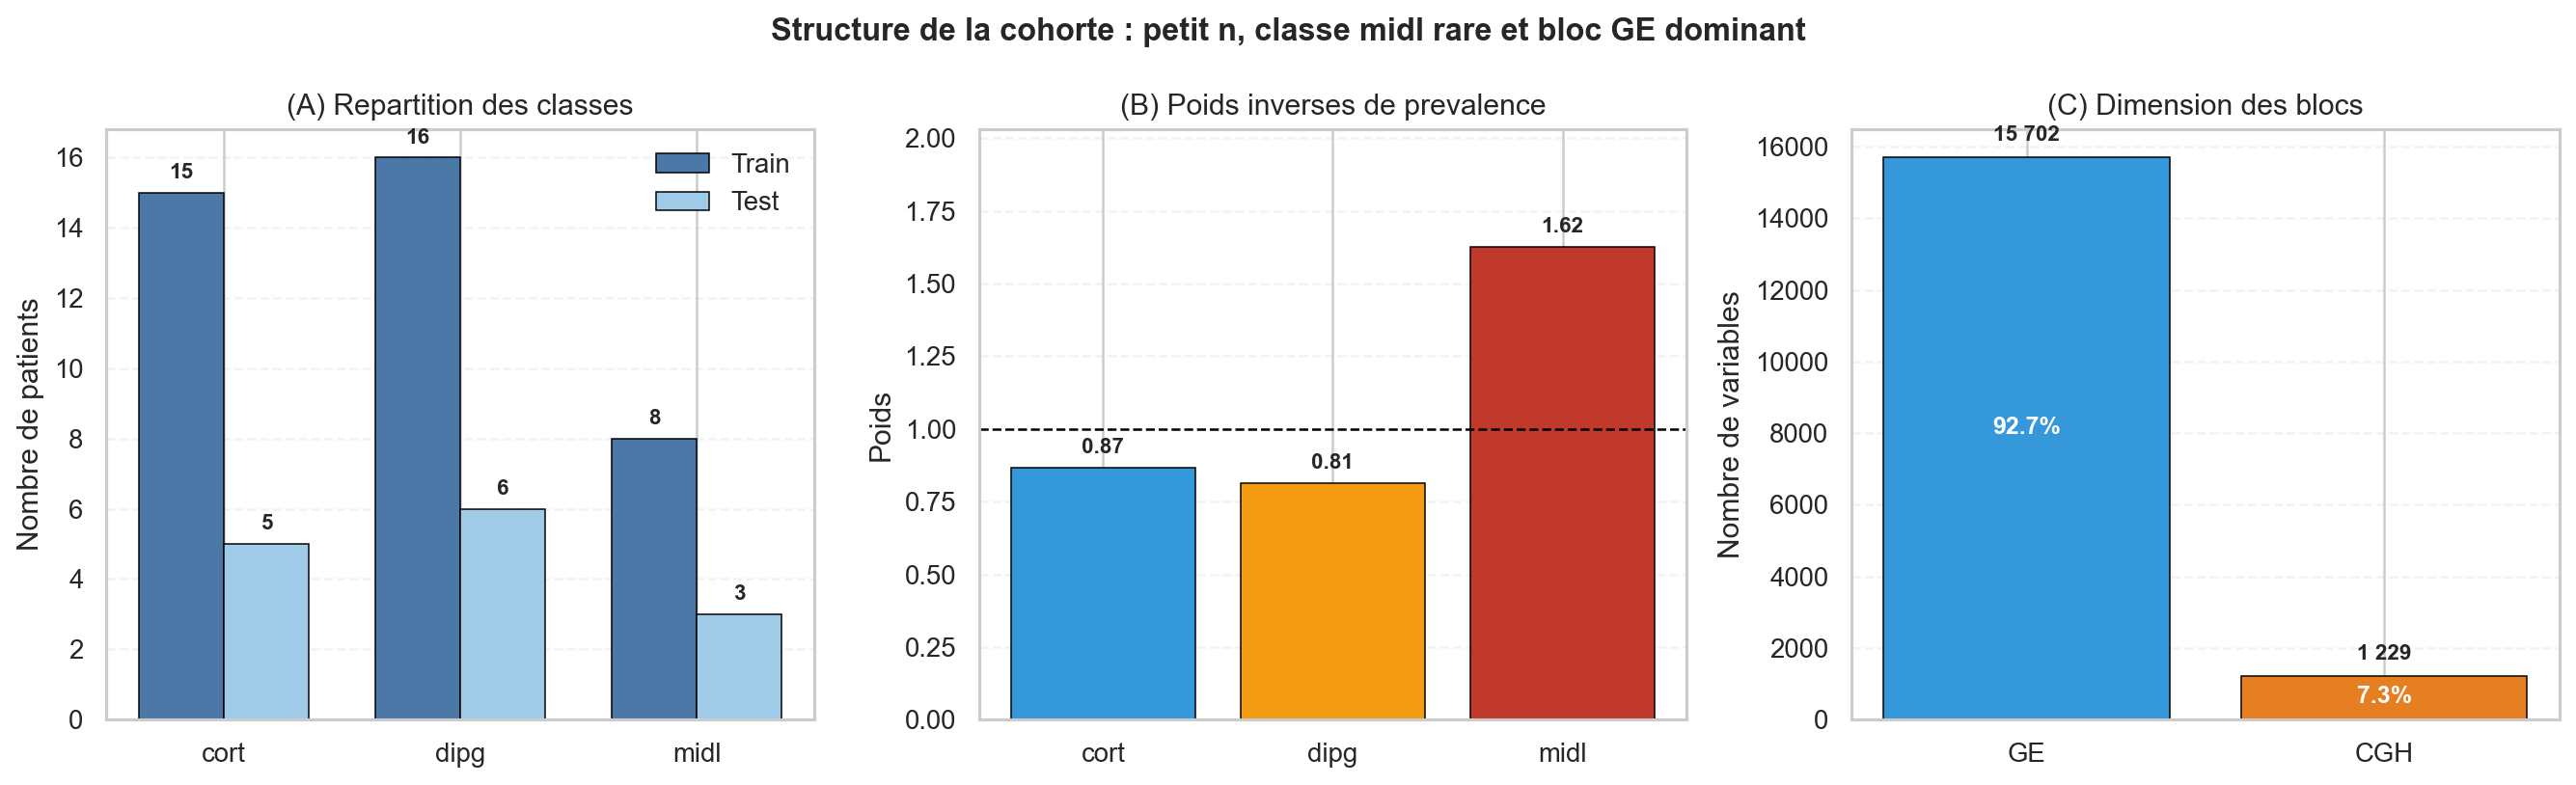
\includegraphics[width=\linewidth]{fig0_eda_cohort.png}
    \caption{\textbf{(A)} Sample counts per class across train and test sets. \textbf{(B)} Inverse prevalence weights
        $w_c = n/(K\,n_c)$ used to balance class contributions in the likelihood. \textbf{(C)} Dimensionality of the two blocks:
        GE concentrates $92.7\%$ of total features.}
    \label{fig:eda_cohort}
\end{figure}

\paragraph{Extreme $p \ggg n$ Regime.}
The training cohort contains $n_{\text{train}} = 39$ patients evaluated across $p = 16{,}931$ molecular features ($15{,}702$ GE $+\ 1{,}229$ CGH), yielding an extreme dimensional ratio:
$$
    \frac{p}{n} \;=\; \frac{16{,}931}{39} \;\simeq\; 434.
$$
In this setting, the empirical Gram matrix $X^{\!\top}X$ has rank at most $n - 1 = 38$. It is singular, rendering any unpenalized estimator completely non-identifiable and prone to severe overfitting. This necessitates systematic recourse to $\ell_1$ and $\ell_2$ regularization and sparse feature selection throughout our entire pipeline.

\paragraph{The Minority Class as the Central Bottleneck.}
Class distribution is markedly imbalanced (Figure~\ref{fig:eda_cohort}A): \texttt{cort} ($15$), \texttt{dipg} ($16$), and \texttt{midl} ($8$) in training. The \texttt{midl} class constitutes only $8/39 \simeq 20.5\%$ of the training set and accounts for only $3$ patients in the test set. Consequently, a single classification error on \texttt{midl} alters test recall in increments of $1/3 \simeq 0.33$. The principal modeling challenge of this benchmark does not reside in separating \texttt{cort} from \texttt{dipg}---which are readily distinguishable---but in accurately identifying the rare \texttt{midl} tumors.

To counteract this imbalance within the likelihood, we introduce inverse prevalence weights (Figure~\ref{fig:eda_cohort}B):
$$
    w_c \;=\; \frac{n}{K\, n_c}, \qquad
    w_{\text{cort}} = 0.87,\;\; w_{\text{dipg}} = 0.81,\;\; w_{\text{midl}} = 1.62,
$$
which scale the contribution of each \texttt{midl} patient by a factor of $\simeq 1.6$ relative to baseline (detailed derivation in §\ref{sec:weights}). Cost-sensitive weighting is statistically superior to synthetic oversampling techniques such as SMOTE (which we tested and found unviable): it rebalances the log-likelihood without fabricating artificial synthetic observations in a $16{,}931$-dimensional space, an operation known to be severely unstable when $p \ggg n$.

\begin{remark}[The Rare Class "Safety Net"]
    Under a One-vs-Rest decomposition, a binary \texttt{midl}-vs-rest classifier whose coefficients are shrunk to zero retains an intercept calibrated to the empirical prior prevalence. The resulting predicted baseline probability is:
    $$
        \hat P_{\text{midl}} \;\simeq\; \frac{n_{\text{midl}}}{n} \;=\; \frac{8}{39} \;\simeq\; 0.205,
    $$
    which remains constant across all patients. Whenever \texttt{cort} and \texttt{dipg} classifiers simultaneously reject an ambiguous observation, this baseline floor can win the final prediction via \texttt{argmax}. This mechanism explains why OvR pipelines successfully recover $2/3$ of test \texttt{midl} patients, whereas the multinomial formulation, constrained by $\sum_c P_c = 1$, captures $0/3$ (cf. Section~\ref{sec:resultats}).
\end{remark}

\paragraph{Dimensional Dominance of the GE Block.}
The GE block accounts for $92.7\%$ of total variables versus $7.3\%$ for CGH (Figure~\ref{fig:eda_cohort}C). Following variable-wise standardization to unit variance, total block inertia scales proportionally with the number of variables $p_j$. The unweighted concatenated matrix $[\,\text{GE}\,|\,\text{CGH}\,]$ is over $90\%$ dominated by GE variance. Any naive concatenation model disproportionately favors GE while discarding CGH. This imbalance motivates the block-wise scaling $\tilde X_j = X_j/\sqrt{p_j}$ used in SGCCA (Section~\ref{sec:sgcca}), which normalizes the initial inertia of each block to unity.

\subsection{Data Quality and Preprocessing}

\paragraph{Missing Data and Variance.}
Inspection of both molecular matrices revealed sparse missing entries and no uninformative zero-variance features following imputation. Consistent with leak-free modeling principles, missing values are imputed using the column-wise median computed exclusively on the training set and subsequently mapped onto test data, avoiding any information leakage.

\paragraph{GE Data Distribution and Scaling.}
The global distribution of the $39 \times 15{,}702$ gene expression measurements (Figure~\ref{fig:eda_ge_dist}) is approximately symmetric, centered ($\text{median} = 0.03$), and bounded ($\min = -10.43$, $\max = 9.87$). Because the data are pre-normalized log-ratios, non-linear transformations (such as logarithmic or Box-Cox transforms) are unnecessary; standard $z$-score scaling suffices prior to scale-sensitive algorithms (PCA, SGCCA).

\begin{figure}[H]
    \centering
    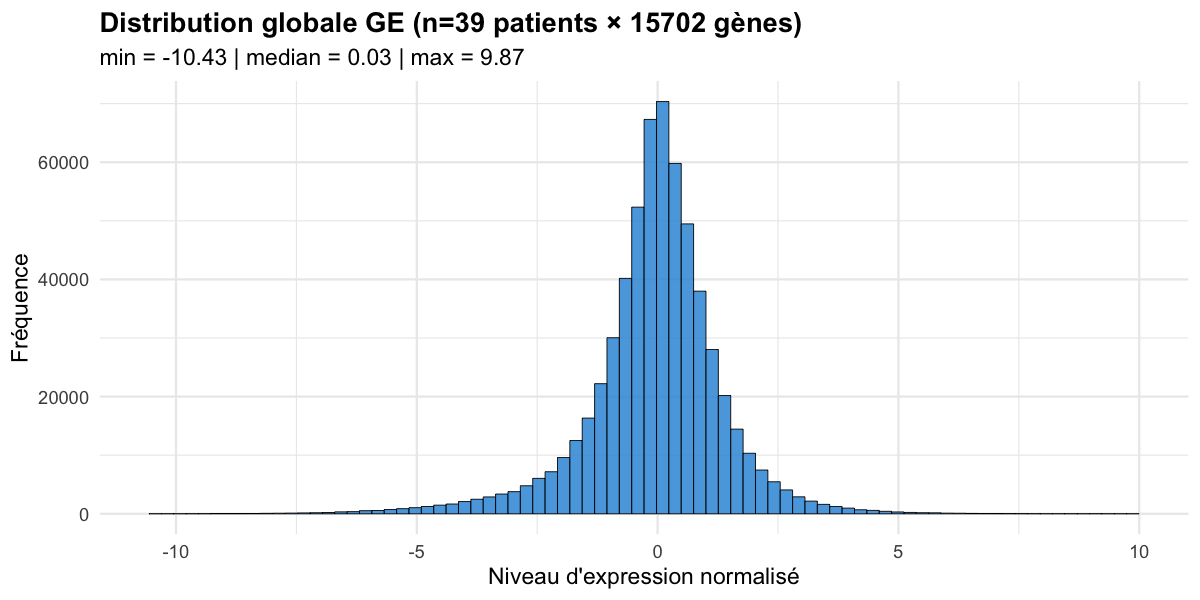
\includegraphics[width=0.78\linewidth]{eda_ge_distribution.png}
    \caption{Global distribution of GE expression levels ($n = 39$ patients $\times\ 15{,}702$ genes).
        The distribution is centered and approximately symmetric: values represent pre-normalized log-ratios, confirming that $z$-score standardization is appropriate.}
    \label{fig:eda_ge_dist}
\end{figure}

\paragraph{Train/Test Covariate Shift.}
Given the small test size ($n = 14$), we evaluated the standardized mean difference (SMD) between train and test distributions feature-by-feature using training statistics. The distribution of $|\text{SMD}|$ is well-behaved across the vast majority of features, ruling out massive systematic covariate shift. The primary source of empirical variance remains the small sample size, underscoring the necessity of repeated cross-validation rather than single validation splits (§\ref{sec:cv}).

\subsection{Unsupervised Separability: Block-Wise PCA}

\begin{figure}[H]
    \centering
    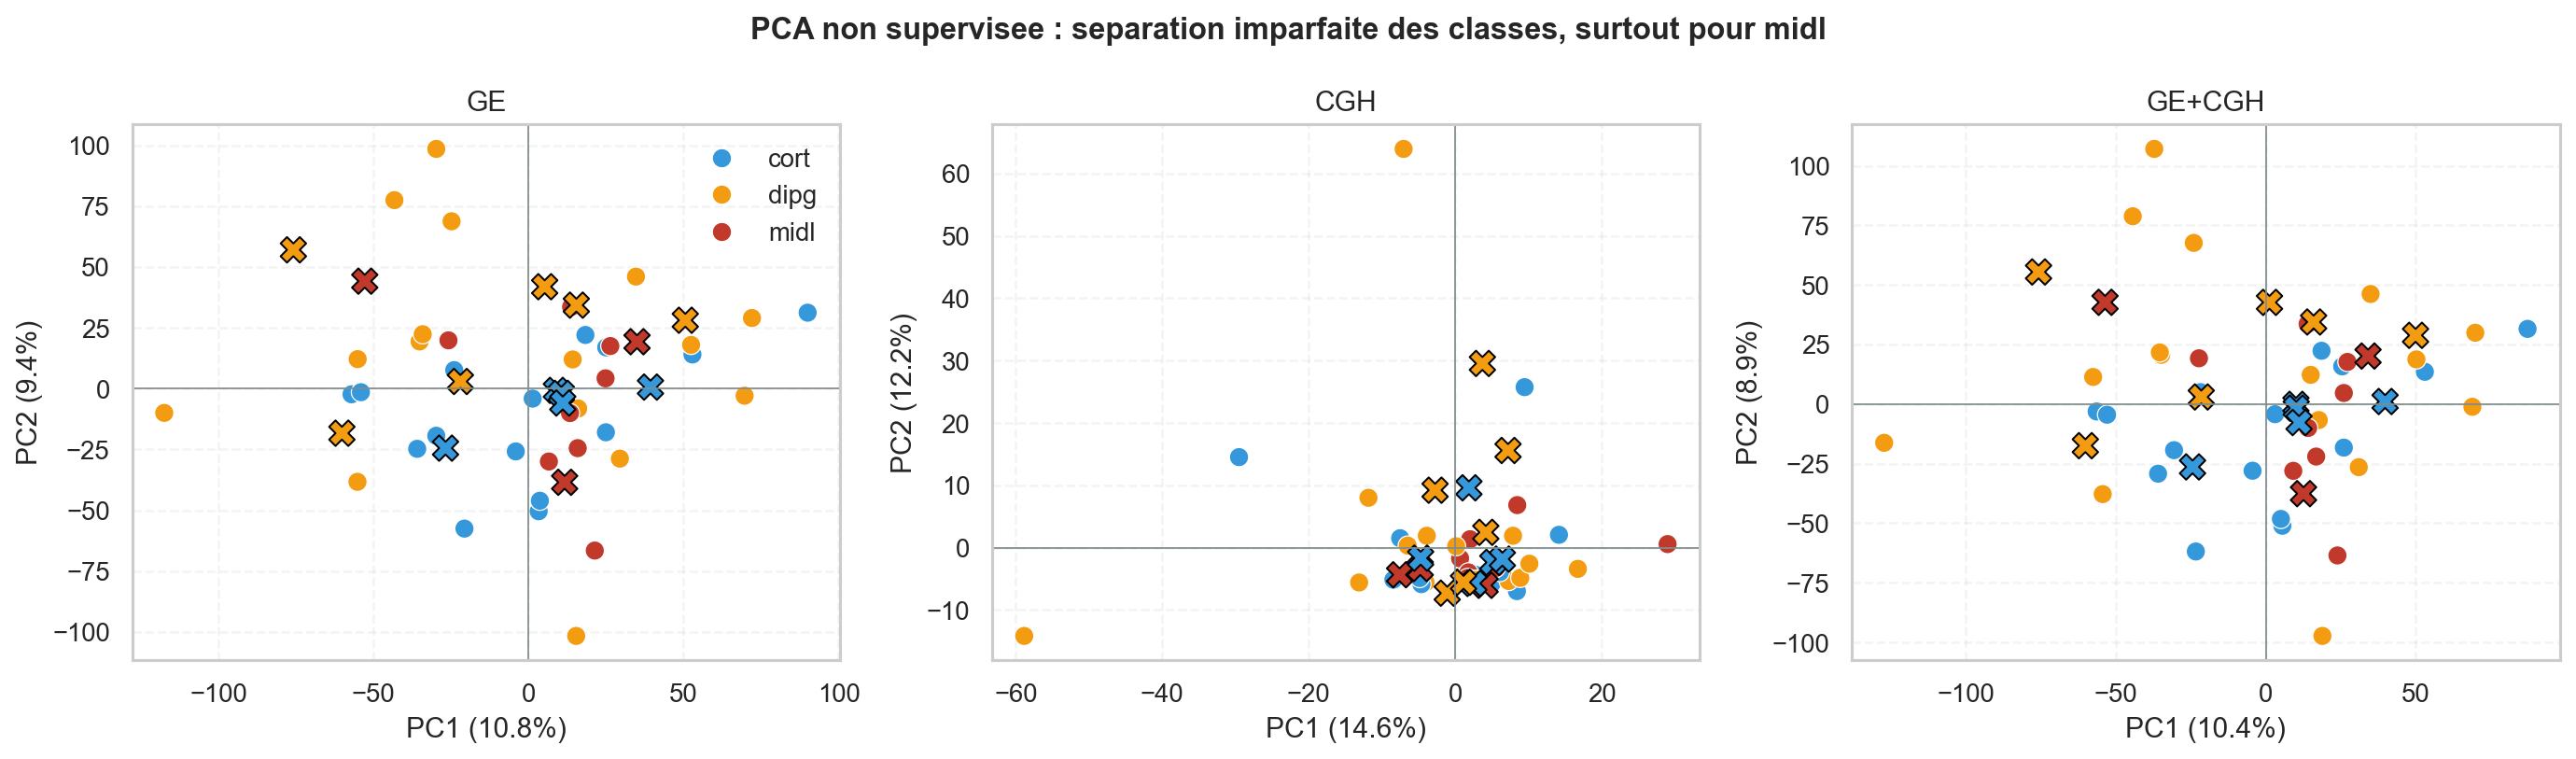
\includegraphics[width=\linewidth]{fig0_eda_pca.png}
    \caption{Unsupervised PCA (first two principal components) across GE, CGH, and concatenated GE+CGH blocks (circles: train; crosses: test). The three classes overlap substantially, particularly \texttt{midl}, with the first two components capturing only a modest fraction of total variance.}
    \label{fig:eda_pca}
\end{figure}

Principal Component Analysis (PCA) addresses a fundamental question: are the clinical classes linearly separable without supervision? The empirical answer is unambiguously negative (Figure~\ref{fig:eda_pca}). The top two principal components capture only a small fraction of total inertia---PC1 + PC2 $\simeq 20\%$ for GE ($10.8\% + 9.4\%$) and $\simeq 27\%$ for CGH ($14.6\% + 12.2\%$)---and the class point clouds exhibit severe overlap. The \texttt{midl} class forms no identifiable cluster, remaining scattered among \texttt{cort} and \texttt{dipg} samples.

\begin{remark}
    The absence of unsupervised clustering carries an important methodological implication: unsupervised dimensionality reduction (PCA, Sparse PCA) projects variance along axes unrelated to the separation of \texttt{midl}. This explains why pipelines pairing \texttt{Sparse PCA + LogReg} failed completely in our benchmarks. Supervised latent projections (such as SGCCA, which explicitly correlates molecular blocks with target class labels) are required to uncover discriminative manifolds.
\end{remark}

\subsection{Correlation Structure and Redundancy}

\begin{figure}[H]
    \centering
    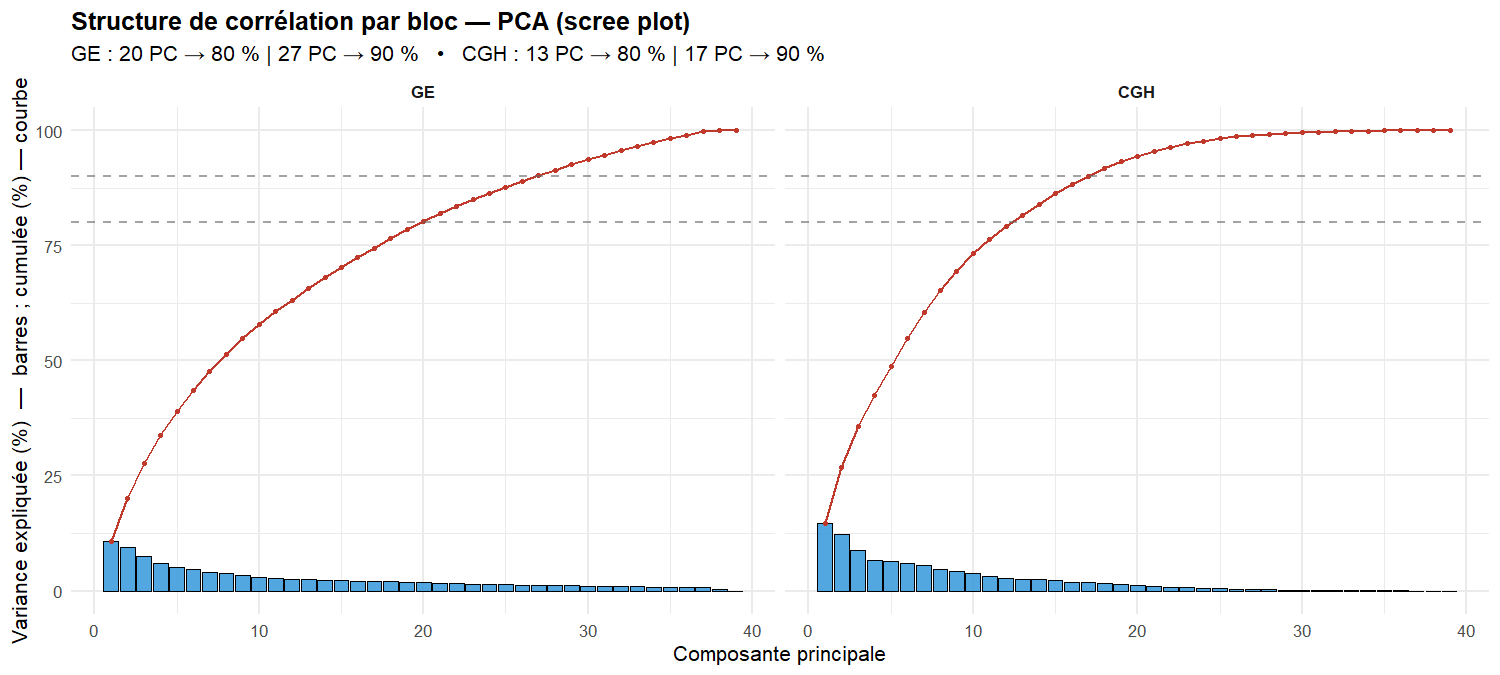
\includegraphics[width=0.95\linewidth]{eda_pca_scree.png}
    \caption{Scree plot per block: explained variance per component (bars) and cumulative variance (red curve), with $80\%$ and $90\%$ thresholds marked by dashed lines. In the $p \ggg n$ regime, rank is bounded by $n-1 = 38$; the concentration rate of variance reflects intra-block collinearity and effective dimensionality.}
    \label{fig:eda_pca_scree}
\end{figure}

In the $p \ggg n$ regime, a large proportion of features are collinear. Rather than displaying an uninterpretable correlation heatmap of randomly subsampled features across thousands of columns, we summarize redundancy via block-wise scree plots (Figure~\ref{fig:eda_pca_scree}). Both blocks possess an effective dimensionality far lower than their nominal feature counts (rank $\le 38$): 20 components are required to capture $80\%$ of GE variance ($27$ for $90\%$), whereas only 13 components capture $80\%$ of CGH variance ($17$ for $90\%$). Redundancy is more pronounced in CGH, consistent with contiguous genomic copy-number alterations, whereas GE distributes variance across broader biological pathways.

This collinearity has two direct consequences:
\begin{itemize}
    \item It favors an Elastic-Net penalty over pure Lasso: the $\ell_2$ component stabilizes coefficient paths among collinear features, whereas pure Lasso arbitrarily selects a single representative feature;
    \item It explains the numerical divergence of Newton solvers in Cooperative Learning for $\rho > 0$: the Hessian $X^{\!\top}WX$ is ill-conditioned, and the agreement term $\rho\,X^{\!\top}X$ amplifies existing collinearity by a factor of $(1+\rho)$ (cf. Section~\ref{sec:resultats}).
\end{itemize}

\subsection{Univariate Signal Around \texttt{midl}}

\begin{figure}[H]
    \centering
    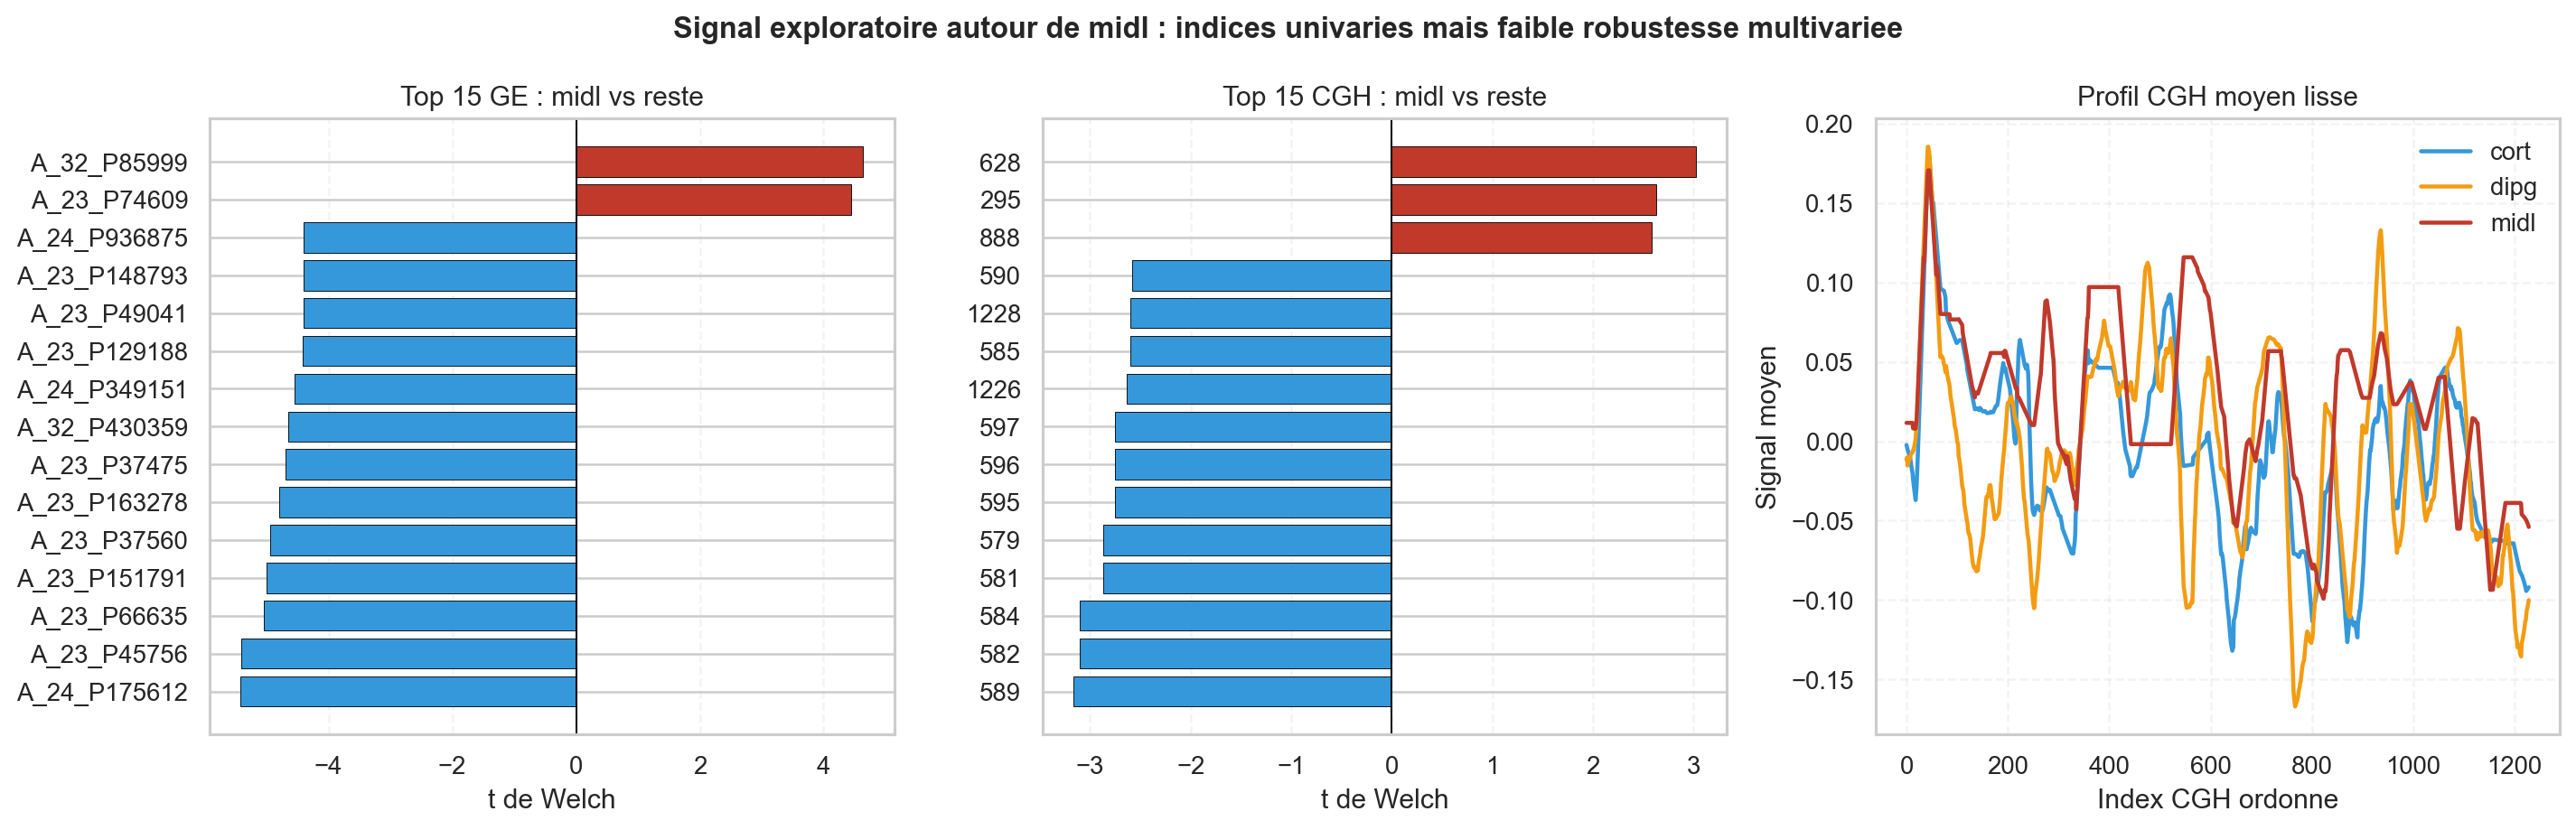
\includegraphics[width=\linewidth]{fig0_eda_midl_signal.png}
    \caption{Left and Center: Top 15 GE and CGH features ranked by absolute Welch's $t$ for the \texttt{midl} vs. rest contrast (red: over-expressed in \texttt{midl}). Right: Mean chromosomal profile smoothed per class along the ordered genomic coordinates.}
    \label{fig:eda_midl}
\end{figure}

To evaluate whether informative univariate signal exists for the rare class, we computed Welch's $t$-statistics for the \texttt{midl}-vs-rest contrast (Figure~\ref{fig:eda_midl}). Welch's $t$-test is chosen over Student's test because it does not assume homoscedasticity, an assumption violated when comparing $n_{\text{midl}} = 8$ against $n_{\text{rest}} = 31$:
\begin{itemize}
    \item \textbf{GE}: several genes attain $|t| \simeq 4$--$5$ (e.g., \texttt{A\_32\_P85999}, over-expressed in \texttt{midl}), while the majority of significant probes are under-expressed. A distinct univariate signal is present.
    \item \textbf{CGH}: test statistics plateau near $|t| \simeq 3$, indicating substantially weaker signal. This explains why data-driven sparse models exclude CGH features.
    \item \textbf{CGH Spatial Profiles}: mean regional copy-number profiles across classes show broad overlap along the genome (Figure~\ref{fig:eda_midl}, right), with no localized region cleanly distinguishing \texttt{midl}.
\end{itemize}

\begin{remark}[Univariate Signal vs. Multivariate Robustness]
    The presence of univariate signal does not guarantee robust multivariate generalization. With $p \ggg n$ and $n_{\text{midl}} = 8$, $t$-statistics exhibit high sampling variance and fail to correct for the multiplicity of $\sim 17{,}000$ hypotheses. While univariate tests highlight candidate biological markers, feature selection must be performed by regularized multivariate estimators within cross-validation.
\end{remark}

\subsection{Evaluation Metric Selection}

\begin{figure}[H]
    \centering
    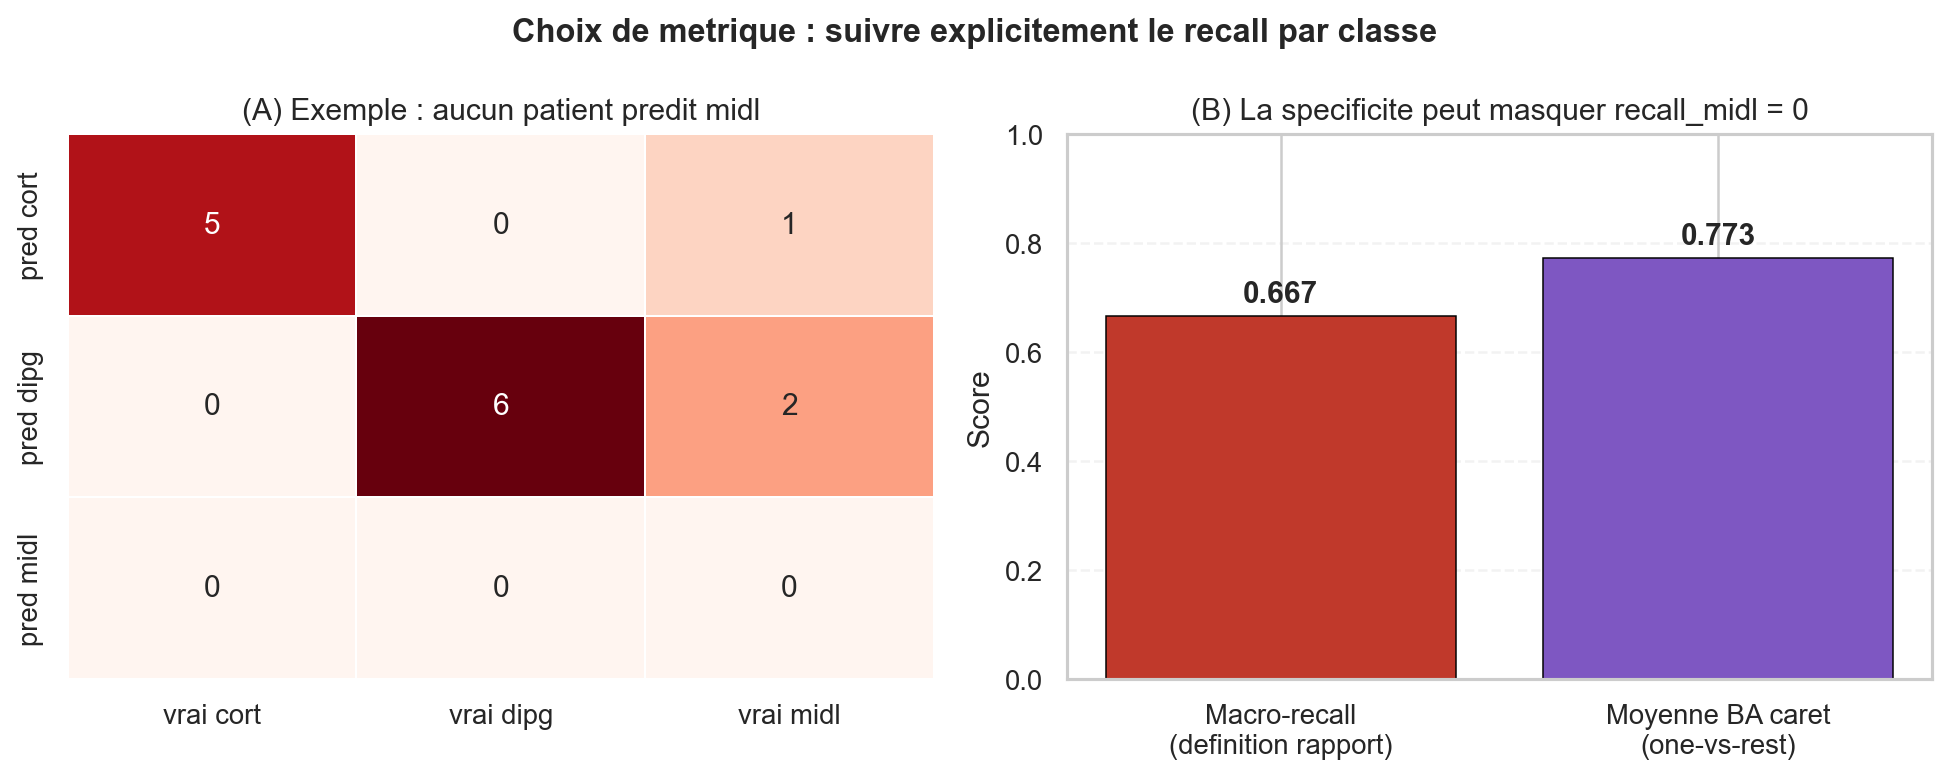
\includegraphics[width=0.92\linewidth]{fig0_eda_metric.png}
    \caption{\textbf{(A)} Confusion matrix of a trivial classifier predicting zero \texttt{midl} cases ($\text{recall}_{\text{midl}} = 0$). \textbf{(B)} The identical prediction scores a macro-recall of $0.667$ but a One-vs-Rest balanced accuracy (as computed by \texttt{caret}) of $0.773$, artificially masking total failure on \texttt{midl}.}
    \label{fig:eda_metric}
\end{figure}

Class imbalance mandates an uncompromised evaluation metric. Raw overall accuracy is uninformative because it implicitly weights classes by prevalence: a naive baseline predicting only \texttt{cort} and \texttt{dipg} already achieves $11/14 \simeq 78.6\%$ test accuracy. We therefore adopt \textbf{macro-recall} (balanced accuracy), defined as the arithmetic mean of class-specific recalls:
\[
    \mathrm{BA}(\hat f) \;=\; \frac{1}{|\mathcal{Y}|}\sum_{c \in \mathcal{Y}} \text{recall}_c(\hat f),
\]
which assigns equal weight to each clinical localization.

A subtle pitfall must be noted regarding the \texttt{caret} implementation in \texttt{R} (Figure~\ref{fig:eda_metric}). In \texttt{caret}, \texttt{mean(cm\$byClass[,"Balanced Accuracy"])} averages binary One-vs-Rest balanced accuracies, which incorporate class specificity. Because the specificity for a rare class remains high even when recall is zero, \texttt{caret}'s metric overestimates model performance:
$$
    \text{macro-recall} = \tfrac{1}{3}\!\left(\tfrac{5}{5} + \tfrac{6}{6} + \tfrac{0}{3}\right) = 0.667,
    \qquad
    \text{BA caret (OvR)} = 0.773.
$$
The \texttt{caret} metric reports an inflated score ($+0.10$), obscuring the complete failure on \texttt{midl}. Throughout this report, we evaluate models based on true macro-recall alongside full confusion matrices.

\subsection{Methodological Synthesis}
Our exploratory analysis establishes the structural constraints of the learning task:
\begin{itemize}
    \item The $p \ggg n$ regime requires strong regularized shrinkage and embedded variable selection.
    \item Severe class imbalance necessitates likelihood weighting and balanced accuracy optimization.
    \item The failure of unsupervised dimension reduction necessitates supervised projection methods (SGCCA, LDA).
    \item The dimensional dominance of GE ($92.7\%$ of variables) requires block-specific scaling prior to multi-omic integration.
\end{itemize}

\newpage


\section{Mathematical Formalism}
\label{sec:formalism}

\subsection{Cross-Entropy and Information Theory\texorpdfstring{\protect\footnote{This section is based on the Information Theory course, CentraleSupélec.}}{}}

Cross-entropy quantifies the divergence between two probability distributions. Given a true discrete distribution $P$ and an estimated model distribution $Q$ defined over a common support $\mathcal{X}$, the cross-entropy of $Q$ relative to $P$ is:
$$H(P, Q) = - \sum_{x \in \mathcal{X}} P(x) \log Q(x).$$
Conceptually, $H(P,Q)$ represents the expected code length required to encode events drawn from $P$ using an optimal code constructed for $Q$. Minimizing cross-entropy is strictly equivalent to minimizing the Kullback-Leibler divergence:
$$D_{\mathrm{KL}}(P \parallel Q) = \sum_{x \in \mathcal X} P(x) \log \frac{P(x)}{Q(x)} = H(P, Q) - H(P).$$

\subsection{Problem Formulation\texorpdfstring{\protect\footnote{This section is based on the Theoretical Machine Learning course, ENSAE.}}{}}

Consider a 3-class classification problem. We observe a training dataset $\mathcal{D} := \{ (X_1, Y_1), \dots, (X_n, Y_n) \}$ with $n = 39$, where each feature vector $X_i \in \mathcal{X} = \mathbb{R}^p$ ($p = 16{,}931$) is paired with an anatomical localization label $Y_i \in \mathcal{Y} = \{1, 2, 3\}$. Pairs $(X_i, Y_i)$ are assumed to be independent and identically distributed (i.i.d.) according to an unknown joint distribution $\mathbb{P}$.

A classifier is a measurable mapping $f : \mathcal{X} \to \mathcal{Y}$. Given a loss function $\ell : \mathcal{Y} \times \mathcal{Y} \to \mathbb{R}$, the theoretical risk of $f$ is:
$$\mathcal{R}(f) := \mathbb{E}_{(X, Y) \sim \mathbb{P}} \big[ \ell\big(f(X), Y\big) \big].$$
The population risk is estimated using an independent test set $\mathcal{D}'_m = \{ (X_1', Y_1'), \dots, (X_m', Y_m') \}$ ($m = 14$):
$$\frac{1}{m}\sum_{i=1}^m \ell\big(f(X_i'), Y_i'\big) \xrightarrow[m \to \infty]{\text{a.s.}} \mathcal{R}(f).$$

The Bayes optimal classifier minimizes the population risk:
$$f^* = \arg\min_f \mathcal{R}(f), \qquad \mathcal{R}^* = \mathcal{R}(f^*).$$

Let $\eta_c(x) = \mathbb{P}[Y = c \mid X = x]$ denote the posterior class probability for $c \in \mathcal{Y}$. Under zero-one loss $\ell(y, y') = \mathbf{1}_{y \ne y'}$, the risk corresponds to classification error probability, and the Bayes decision rule is:
$$f^*(x) = \arg\max_{c \in \mathcal{Y}} \eta_c(x).$$

\begin{proof}
    For any classifier $f$, the risk under zero-one loss satisfies:
    \begin{align*}
        \mathcal{R}(f) & = \mathbb{E}_{(X, Y)}\big[\mathbf{1}_{f(X) \ne Y}\big] = \mathbb{E}_X\Big[\mathbb{E}_{Y \mid X}\big[\mathbf{1}_{f(X) \ne Y}\big]\Big] \\
                       & = \mathbb{E}_X\big[\mathbb{P}(f(X) \ne Y \mid X)\big].
    \end{align*}
    Minimizing the outer expectation is achieved by pointwise minimization for each fixed $x \in \mathcal{X}$. Letting $\hat y = f(x)$:
    $$\mathbb{P}(\hat y \ne Y \mid X = x) = 1 - \mathbb{P}(Y = \hat y \mid X = x) = 1 - \eta_{\hat y}(x).$$
    Minimizing error probability is therefore equivalent to maximizing $\eta_{\hat y}(x)$, yielding:
    \[
        f^*(x) = \arg\max_{c \in \mathcal{Y}} \eta_c(x).
    \]
\end{proof}

\begin{remark}
    This result holds specifically for symmetric zero-one loss. Under asymmetric cost structures (e.g., penalizing misclassifications of rare \texttt{midl} tumors more heavily), the Bayes predictor deviates from the standard argmax of unweighted posterior probabilities.
\end{remark}

\subsection{Multiclass Logistic Regression\texorpdfstring{\protect\footnote{This section is based on the Theoretical Machine Learning and Optimization courses, ENSAE.}}{}}
\label{sec:logreg}

Because direct minimization of empirical zero-one loss is NP-hard, multinomial logistic regression employs empirical cross-entropy as a smooth, convex surrogate loss. The class probabilities are parameterized using the softmax function:
$$\eta_c^\beta(x) = \mathbb{P}_\beta[Y = c \mid X = x] = \frac{e^{\beta_c^\top x}}{\sum_{k=1}^3 e^{\beta_k^\top x}},$$
where $\beta = (\beta_1, \beta_2, \beta_3) \in \mathbb{R}^{p \times 3}$. To ensure parameter identifiability against translational shifts $\beta_c \mapsto \beta_c + \gamma$, we enforce the standard reference constraint $\beta_3 = 0$.

For i.i.d. observations, the likelihood function is:
$$\mathcal{L}(\beta) = \prod_{i=1}^n \prod_{c=1}^3 \big(\eta_c^\beta(X_i)\big)^{\mathbf{1}_{Y_i=c}}.$$
The log-likelihood $\ell(\beta) = \log \mathcal{L}(\beta)$ expands as:
$$\ell(\beta) = \sum_{i=1}^n \left( \beta_{Y_i}^\top X_i - \log\left(\sum_{k=1}^3 e^{\beta_k^\top X_i}\right) \right).$$
Maximizing log-likelihood is equivalent to minimizing the empirical cross-entropy risk:
$$\hat{R}_n(\beta) = -\frac{1}{n} \sum_{i=1}^n \log \eta_{Y_i}^\beta(X_i).$$
The function $\beta \mapsto \hat{R}_n(\beta)$ is convex and continuously differentiable.

\subsubsection{Weighted Likelihood and Optimal Class Weights}
\label{sec:weights}

Standard empirical risk $\hat R_n$ assigns uniform weight $1/n$ to every patient. Because \texttt{midl} represents only $n_{\text{midl}}/n = 8/39 \simeq 20.5\%$ of the cohort, minimizing unweighted risk permits the majority classes to dominate. To align empirical optimization with macro-recall, we formulate the \textbf{weighted empirical risk}:
$$
    \hat{R}_n^{\,w}(\beta) \;=\; -\frac{1}{n} \sum_{i=1}^n w_{Y_i}\,\log \eta_{Y_i}^\beta(X_i),
$$
where observation weights $w_{Y_i} > 0$ depend exclusively on class membership.

\paragraph{Derivation of Inverse Prevalence Weights.}
Let $n_c$ denote the number of training instances belonging to class $c$. The total contribution of class $c$ to the objective is proportional to $w_c n_c$. Setting class contributions to be equal across all $K$ classes:
$$
    w_c\, n_c \;=\; \text{constant} \quad \forall c \in \{1,\dots,K\},
$$
and normalizing such that the mean observation weight equals unity ($\sum_c w_c n_c = n$):
$$
    \boxed{\,w_c \;=\; \frac{n}{K\, n_c}\,}.
$$
Substituting our cohort counts ($n = 39, K = 3$):
$$
    w_{\text{cort}} = \frac{39}{3 \times 15} \simeq 0.87,\qquad
    w_{\text{dipg}} = \frac{39}{3 \times 16} \simeq 0.81,\qquad
    w_{\text{midl}} = \frac{39}{3 \times 8} \simeq 1.62.
$$
Each \texttt{midl} patient carries approximately double the weight of a \texttt{dipg} patient. This corresponds to the standard \texttt{class\_weight="balanced"} parameterization.

\paragraph{Gradient and Optimization.}
The gradient of the weighted empirical risk with respect to $\beta_c$ is:
$$
    \nabla_{\beta_c} \hat{R}_n^{\,w}(\beta) = \frac{1}{n} \sum_{i=1}^n w_{Y_i}\left( \eta_c^\beta(X_i) - \mathbf{1}_{\{Y_i = c\}} \right) X_i.
$$
Residuals for \texttt{midl} instances are magnified by $w_{\text{midl}}$, penalizing misclassifications on the rare class. Convexity is preserved, ensuring global convergence.

In practical implementations, the stationary condition $\nabla_\beta \hat R_n^w(\beta) = 0$ is solved using iteratively reweighted least squares (IRLS) via Newton-Raphson updates or proximal coordinate descent:
$$\beta_c^{(t+1)} = \beta_c^{(t)} - \gamma_t \nabla_{\beta_c} \hat R_n^w(\beta^{(t)}).$$

Following convergence to the optimal parameter estimates $\hat \beta$, prediction for a new test instance $x$ is given by:
$$\hat{y} = \arg\max_{c \in \mathcal{Y}} \eta_c^{\hat{\beta}}(x) = \arg\max_{c \in \{1, 2, 3\}} \big(\hat{\beta}_c^\top x\big),$$
which defines linear decision boundaries in $\mathbb{R}^p$.

\subsection{Penalized Empirical Risk: Elastic-Net Regularization\texorpdfstring{\protect\footnote{This section is based on the Statistics course, CentraleSupélec.}}{}}

In the $p \gg n$ regime, unregularized maximum likelihood overfits severely. We introduce an Elastic-Net penalty combining $\ell_1$ (Lasso) and $\ell_2$ (Ridge) regularizers:
$$\min_{\beta} \bigg( \hat R_n^w(\beta) + \lambda \alpha \|\beta\|_1 + \frac{\lambda (1 - \alpha)}{2} \|\beta\|_2^2 \bigg),$$
where $\lambda > 0$ governs overall regularization strength and $\alpha \in [0, 1]$ tunes the balance between sparsity ($\alpha = 1$, Lasso) and coefficient shrinkage ($\alpha = 0$, Ridge).

Because the $\ell_1$ norm is non-differentiable at the origin, optimization is performed using proximal operators. Coordinate updates apply the soft-thresholding operator:
$$\mathcal{S}(v, \tau) = \operatorname{sign}(v)\max(|v| - \tau, 0),$$
which drives uninformative coefficients to exactly zero, producing sparse, interpretable biomarker signatures.

\subsection{Generalized Linear Models (GLM)\texorpdfstring{\protect\footnote{This section is based on the Big Data \& Health (CentraleSupélec) and Theoretical Machine Learning (ENSAE) courses.}}{}}

A Generalized Linear Model posits that the conditional distribution $Y_i \mid X_i = x_i$ belongs to the exponential dispersion family:
$$f_{Y_i}(y_i \mid \theta_i, \phi) = \exp\left( \frac{y_i \theta_i - b(\theta_i)}{a(\phi)} + c(y_i, \phi) \right),$$
where $\theta_i$ is the natural parameter, $\phi$ is the dispersion parameter, and $b(\cdot)$ is the cumulant function. The conditional moments satisfy:
$$\mathbb{E}[Y_i \mid X_i = x_i] = b'(\theta_i) =: \mu_i, \qquad \operatorname{Var}(Y_i \mid X_i = x_i) = b''(\theta_i) a(\phi) = V(\mu_i) a(\phi).$$

The link function $g(\cdot)$ connects the conditional mean $\mu_i$ to the linear predictor $\eta_i = x_i^\top \beta$:
$$g(\mu_i) = x_i^\top \beta.$$
When $g = (b')^{-1}$, the link is canonical ($\eta_i = \theta_i$), ensuring strict concavity of the log-likelihood.

For categorical classification with $K \ge 2$ classes, $Y \mid X = x \sim \text{Categorical}(\mu_1(x), \dots, \mu_K(x))$ with $\sum_{c=1}^K \mu_c = 1$. Representing $Y$ as a one-hot vector $(Y_1, \dots, Y_K)^\top$, the density is:
$$f_Y(y \mid x) = \prod_{c=1}^K \mu_c(x)^{y_c} = \exp\left( \sum_{c=1}^{K-1} y_c \log \frac{\mu_c(x)}{\mu_K(x)} + \log \mu_K(x) \right),$$
which is a multivariate exponential family with natural parameter vector $\theta_c(x) = \log(\mu_c(x)/\mu_K(x))$. Under the linear canonical link $\theta_c(x) = x^\top \beta_c$ with $\beta_K = 0$, we recover the softmax multinomial model:
$$\mu_c(x) = \frac{e^{x^\top \beta_c}}{1 + \sum_{k=1}^{K-1} e^{x^\top \beta_k}} = \text{softmax}_c(x^\top \beta).$$

\subsection{Linear Discriminant Analysis (LDA)}

The Bayes classifier maximizes posterior probability $\mathbb{P}[Y = c \mid X = x] \propto \pi_c f_c(x)$, where $\pi_c = \mathbb{P}[Y = c]$ is the class prior and $f_c$ is the class-conditional density. LDA assumes:
\begin{itemize}
    \item \textbf{Class-conditional normality}: $X \mid Y = c \sim \mathcal{N}_p(\mu_c, \Sigma_c)$;
    \item \textbf{Homoscedasticity}: $\Sigma_c = \Sigma$ for all $c \in \mathcal{Y}$.
\end{itemize}

Under these assumptions, the quadratic term $-\frac{1}{2}x^\top \Sigma^{-1} x$ is shared across all classes, yielding the linear discriminant function:
$$\delta_c(x) = \log \pi_c - \frac{1}{2}\mu_c^\top \Sigma^{-1}\mu_c + x^\top \Sigma^{-1}\mu_c = \mathbf{w}_c^\top x - b_c,$$
where $\mathbf{w}_c = \Sigma^{-1}\mu_c$ and $b_c = \frac{1}{2}\mu_c^\top \Sigma^{-1}\mu_c - \log \pi_c$.

The parameters are estimated empirically:
$$\hat \pi_c = \frac{n_c}{n}, \qquad \hat \mu_c = \frac{1}{n_c}\sum_{i : Y_i = c} X_i, \qquad \hat \Sigma = \frac{1}{n-K}\sum_{c=1}^K \sum_{i : Y_i = c} (X_i - \hat \mu_c)(X_i - \hat \mu_c)^\top.$$

\begin{remark}[Singularity in High Dimensions]
    In our setting ($p = 16{,}931$ and $n = 39$), $\hat \Sigma$ has rank at most $36$ and is singular. Direct application of LDA to raw feature space is impossible. Instead, LDA is applied to the low-dimensional supervised latent components extracted by SGCCA ($d \ll n$).
\end{remark}

\subsection{Cross-Validation Strategy}
\label{sec:cv}

With $n = 39$, single validation splits exhibit high variance. We employ a stratified, repeated, nested cross-validation protocol.

\paragraph{Stratification.}
Each fold $\mathcal{F}_k$ ($k = 1, \dots, K$) is constructed to preserve empirical class proportions:
$$\frac{|\{i \in \mathcal{F}_k : Y_i = c\}|}{|\mathcal{F}_k|} \simeq \frac{n_c}{n} \quad \forall c \in \mathcal{Y}.$$
This guarantees that the rare class \texttt{midl} is represented within every fold.

\paragraph{Repetitions.}
To reduce partitioning variance, $K$-fold cross-validation ($K = 7$) is repeated across $R = 3$ independent random splits ($K \times R = 21$ total folds):
$$\widehat{\mathcal{R}}_{\mathrm{CV}}(\theta) = \frac{1}{RK} \sum_{r=1}^R \sum_{k=1}^K \frac{1}{|\mathcal{F}_k^{(r)}|} \sum_{i \in \mathcal{F}_k^{(r)}} \ell\big(\hat f^{(-k,r)}_\theta(X_i), Y_i\big).$$

\paragraph{Nested Cross-Validation.}
To tune internal hyperparameters (such as $\lambda$ in \texttt{glmnet} or sparsity parameters in \texttt{RGCCA}) without data leakage, an inner cross-validation loop is executed strictly within each outer training fold:
$$\hat \lambda = \arg\min_\lambda \widehat{\mathcal{R}}_{\text{inner}}(\lambda).$$
The outer test fold remains completely untouched until final evaluation.

\subsection{Multi-Block Fusion Frameworks}

Let $X \in \mathbb{R}^{n \times p_1}$ denote the gene expression block ($p_1 = 15{,}702$) and $Z \in \mathbb{R}^{n \times p_2}$ denote the CGH block ($p_2 = 1{,}229$).

\subsubsection{Baseline Strategies}
\begin{itemize}
    \item \textbf{Early Fusion}: Concatenates $[X \mid Z] \in \mathbb{R}^{n \times (p_1 + p_2)}$. Because GE constitutes $> 90\%$ of variables, it numerically overwhelms the CGH block.
    \item \textbf{Late Fusion}: Trains separate models $f_X$ and $f_Z$, aggregating predictions via convex combination $\omega f_X(X) + (1-\omega) f_Z(Z)$. This ignores cross-modal interactions.
\end{itemize}

\subsubsection{Cooperative Learning}
Cooperative Learning \cite{ding2022cooperative} bridges early and late fusion by penalizing disagreements between block-specific predictions. In multi-class logistic regression, the agreement penalty is applied to predicted linear logits:
$$J(\theta_x, \theta_z) = \hat{R}_{\text{CE}}(\theta_x, \theta_z) + \frac{\rho}{2}\|X\theta_x - Z\theta_z\|_F^2 + \mathcal{P}_{\text{Elastic-Net}}(\theta_x, \theta_z),$$
where $\rho \ge 0$ modulates cross-view agreement ($\rho = 0$ corresponds to early fusion; $\rho \to \infty$ enforces strict consensus).

The optimization problem can be cast into standard Elastic-Net form on an augmented dataset:
$$\tilde{X} = \begin{pmatrix} W^{1/2}X & W^{1/2}Z \\ -\sqrt{\rho}X & \sqrt{\rho}Z \end{pmatrix}, \quad \tilde{z} = \begin{pmatrix} z \\ 0 \end{pmatrix}, \quad \tilde{\beta} = \begin{pmatrix} \theta_x \\ \theta_z \end{pmatrix}.$$

\subsubsection{RGCCA and SGCCA Framework}
\label{sec:sgcca}

Sparse Generalized Canonical Correlation Analysis (SGCCA) \cite{tenenhaus2011rgcca, tenenhaus2014sgcca} seeks sparse block components $y_j = X_j a_j$ that maximize inter-block covariances across connected blocks:
\begin{equation}
    \max_{a_1, \dots, a_J} \sum_{j,k=1}^J c_{jk} \, g\big(\operatorname{cov}(X_j a_j, X_k a_k)\big) \quad \text{s.t.} \quad \|a_j\|_2 \le 1, \; \|a_j\|_1 \le s_j,
    \label{eq:sgcca}
\end{equation}
where $C = (c_{jk})$ is a symmetric design matrix, $g(x) = x^2$, and $s_j \in [1/\sqrt{p_j}, 1]$ controls the sparsity of block weights $a_j$.

\begin{algorithm}[H]
    \caption{Cyclic Block Coordinate Ascent for SGCCA}
    \label{alg:sgcca}
    \KwIn{Data blocks $X_1, \dots, X_J$; design matrix $C$; sparsity bounds $s_j$; tolerance $\varepsilon > 0$}
    \KwOut{Optimal weight vectors $\mathbf{a}_1^*, \dots, \mathbf{a}_J^*$}

    \textbf{Initialization:} Draw $\mathbf{a}_j^{(0)} \in \Omega_j$ with $\|\mathbf{a}_j^{(0)}\|_2 = 1$ for $j = 1, \dots, J$\;
    $t \leftarrow 0$\;

    \Repeat{$\big|f(\mathbf{a}_1^{(t+1)}, \dots, \mathbf{a}_J^{(t+1)}) - f(\mathbf{a}_1^{(t)}, \dots, \mathbf{a}_J^{(t)})\big| < \varepsilon$}{
        \For{$j = 1$ \KwTo $J$}{
            Compute gradient: $\nabla_j f = \sum_{k=1}^J c_{jk} X_j^\top X_k \mathbf{a}_k^{(t)}$\;
            Soft-thresholding update: $\mathbf{a}_j^{(t+1)} \leftarrow \frac{\mathcal{S}(\nabla_j f, \lambda_j)}{\|\mathcal{S}(\nabla_j f, \lambda_j)\|_2}$\;
            Tune $\lambda_j$ to satisfy $\|\mathbf{a}_j^{(t+1)}\|_1 \le s_j$\;
        }
        $t \leftarrow t + 1$\;
    }
\end{algorithm}

To incorporate supervised guidance, we configure $J = 3$ blocks:
$$X_1 = X_{\text{GE}}, \qquad X_2 = X_{\text{CGH}}, \qquad X_3 = Y \in \{0, 1\}^{n \times 3},$$
with the supervised design matrix:
$$
    C = \begin{pmatrix} 0 & 0 & 1 \\ 0 & 0 & 1 \\ 1 & 1 & 0 \end{pmatrix}.
$$
The dummy label matrix $Y$ serves as a supervised pivot: GE and CGH are not constrained to correlate directly with each other, but rather to maximize covariance with the clinical localization classes.

Prior to SGCCA, blocks are standardized and scaled by their degrees of freedom:
$$\tilde X_j = \frac{1}{\sqrt{p_j}} X_j,$$
which guarantees $\operatorname{Tr}(\tilde X_j^\top \tilde X_j) = 1$, equalizing block inertia. The resulting low-dimensional components feed into an LDA classifier.

\newpage


\section{Results}
\label{sec:resultats}

\subsection{Feature Selection and Method Comparison}

\paragraph{SGCCA Parameter Tuning.}
For SGCCA, sparsity parameters $(s_1, s_2)$ were tuned via cross-validation across a grid of candidate configurations using \texttt{RGCCA}. The optimal setting corresponds to \texttt{Set 8} ($s_1 = 0.051$ for GE, $s_2 = 0.067$ for CGH), retaining:
\begin{itemize}
    \item \textbf{68} active features in the GE block;
    \item \textbf{11} active features in the CGH block.
\end{itemize}
The objective criterion at convergence evaluates to $0.0042$. As explained in Section~\ref{sec:sgcca}, this magnitude reflects the $1/\sqrt{p_j}$ normalization applied to equalize block inertia.

\paragraph{Cooperative Learning and Solver Divergence.}
When applying Cooperative Learning via \texttt{multiview} (which wraps \texttt{glmnet}) under a One-vs-Rest formulation, the algorithm diverges for any non-zero agreement penalty $\rho > 0$, throwing repeated non-convergence warnings (\texttt{glmnet.fit: algorithm did not converge}).

This numerical failure stems from two structural factors:
\begin{enumerate}
    \item For the rare \texttt{midl} class, Newton weights $w_i = \hat p_i(1 - \hat p_i)$ approach zero, rendering $X^\top W X$ severely ill-conditioned.
    \item The agreement penalty injects $\rho X^\top X$, amplifying intra-block collinearity by a factor of $(1 + \rho)$.
\end{enumerate}
Consequently, only $\rho = 0$ is computationally viable in the OvR setting, reducing Cooperative Learning to an independent OvR Lasso. Conversely, the multinomial cooperative model converges successfully at $\rho^* = 0.10$, but achieves lower balanced accuracy.

\paragraph{Multinomial vs. One-vs-Rest Formulations.}
In high-dimensional regimes with imbalanced classes, multinomial softmax and One-vs-Rest logistic regressions behave markedly differently:
\begin{itemize}
    \item \textbf{Multinomial Softmax}: Enforces $\sum_c P_c = 1$. When the rare class \texttt{midl} lacks dominant features, the softmax denominator pulls probability mass toward the majority classes (\texttt{dipg}), leading the $\ell_1$ penalty to zero out all \texttt{midl} coefficients. Test recall for \texttt{midl} is $0/3$.
    \item \textbf{One-vs-Rest}: Trains independent binary sub-classifiers. When \texttt{midl} features are zeroed out, the sub-classifier intercept maintains an empirical baseline probability:
          $$\hat P_{\text{midl}} = \sigma(\log(8/31)) \simeq 0.205.$$
          When \texttt{cort} and \texttt{dipg} classifiers simultaneously reject a patient, this baseline probability wins the $\arg\max$ decision, correctly recovering $2/3$ test \texttt{midl} patients.
\end{itemize}

\paragraph{Grouped vs. Ungrouped Penalization.}
Multinomial Lasso supports two $\ell_1$ structures:
\begin{itemize}
    \item \textbf{Grouped}: $\lambda \sum_{j=1}^p \|\beta_{j,\cdot}\|_2$, enforcing shared sparsity across all classes for each gene.
    \item \textbf{Ungrouped}: $\lambda \sum_{j=1}^p \sum_{c=1}^K |\beta_{j,c}|$, allowing class-specific variable selection.
\end{itemize}
Switching from grouped to ungrouped penalization increases CV balanced accuracy by $+0.054$ (from $0.784$ to $0.838$), though test set performance remains identical ($0.773$).

\subsection{Benchmark Performance Synthesis}

\begin{table}[h]
    \centering
    \renewcommand{\arraystretch}{1.15}
    \begin{tabular}{l c c c c}
        \toprule
        \textbf{Method}                    & \textbf{CV bal\_acc} & \textbf{Test bal\_acc} & \textbf{midl test} & \textbf{N$_{\text{vars}}$} \\
        \midrule
        Multinomial Lasso grouped          & $0.784 \pm 0.096$    & $0.773$                & $0/3$              & $27$ GE                    \\
        Multinomial Lasso ungrouped        & $0.838 \pm 0.123$    & $0.773$                & $0/3$              & $27$ GE                    \\
        Cooperative Lasso OvR ($\rho = 0$) & $0.833 \pm 0.129$    & $0.924$                & $2/3$              & $42$ GE                    \\
        SGCCA + LDA                        & $0.829 \pm 0.133$    & $0.924$                & $2/3$              & $68$ GE + $11$ CGH         \\
        \bottomrule
    \end{tabular}
    \caption{Performance comparison across supervised sparse models evaluated on an identical protocol
        (stratified 7-fold CV $\times$ 3, held-out test set $n=14$). The \texttt{midl} test column reports the proportion of correctly classified midline tumors.}
    \label{tab:resultats_finaux}
\end{table}

\begin{figure}[H]
    \centering
    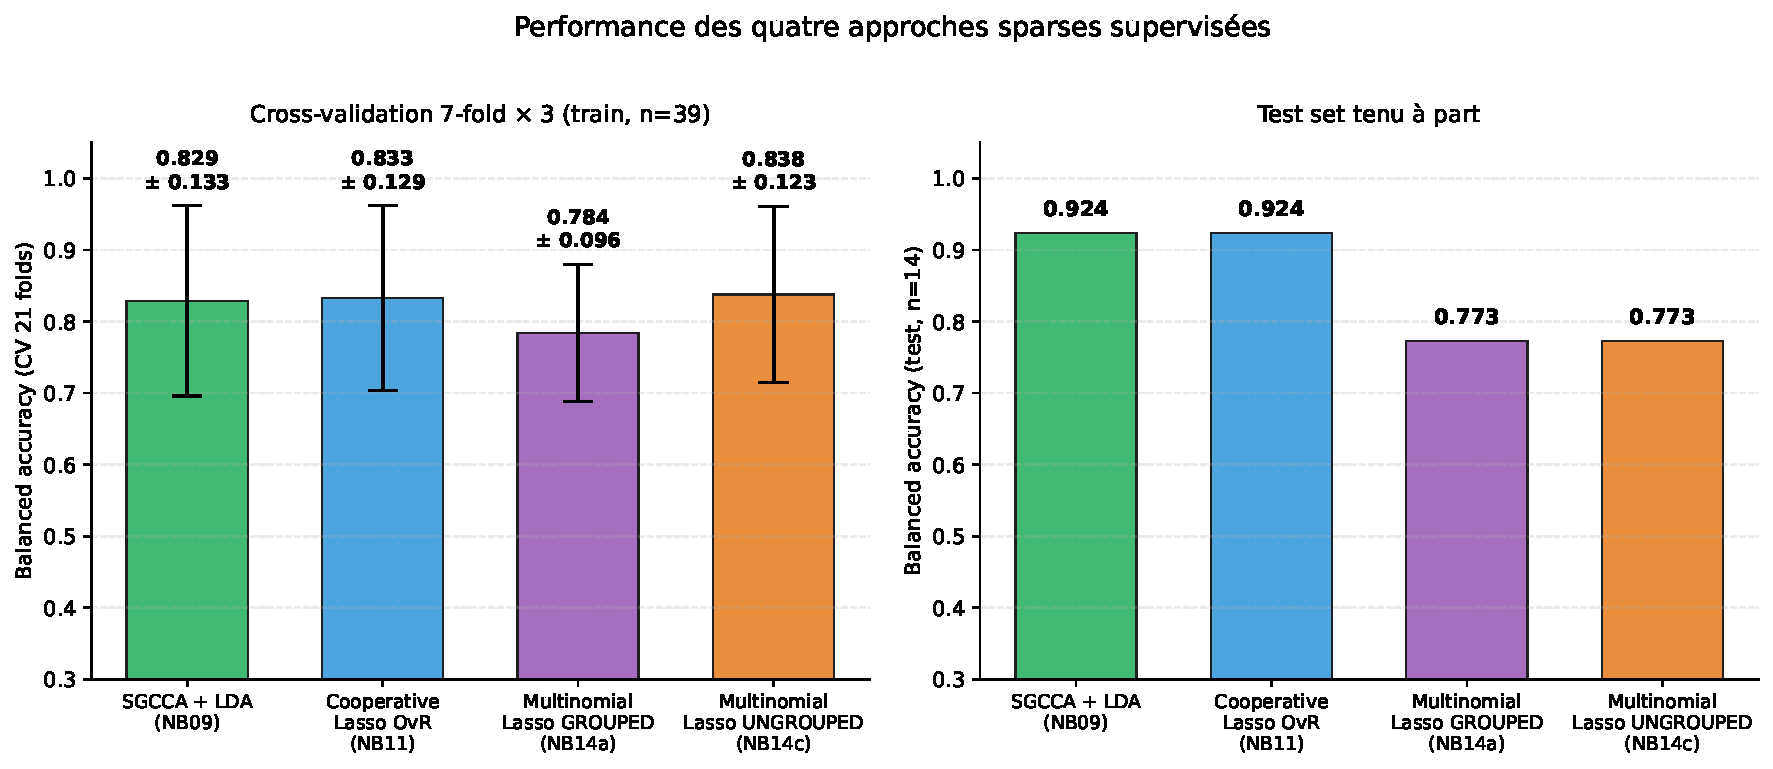
\includegraphics[width=\linewidth]{fig1_comparison.pdf}
    \caption{Comparative performance of the four supervised sparse pipelines. Left: Balanced accuracy in stratified cross-validation ($7\text{-fold} \times 3 = 21$ folds, $n_{\text{train}} = 39$), with error bars indicating one standard deviation. Right: Balanced accuracy on the held-out test set ($n_{\text{test}} = 14$). Only SGCCA + LDA and Cooperative OvR achieve $0.924$ test balanced accuracy.}
    \label{fig:comparison}
\end{figure}

\begin{figure}[H]
    \centering
    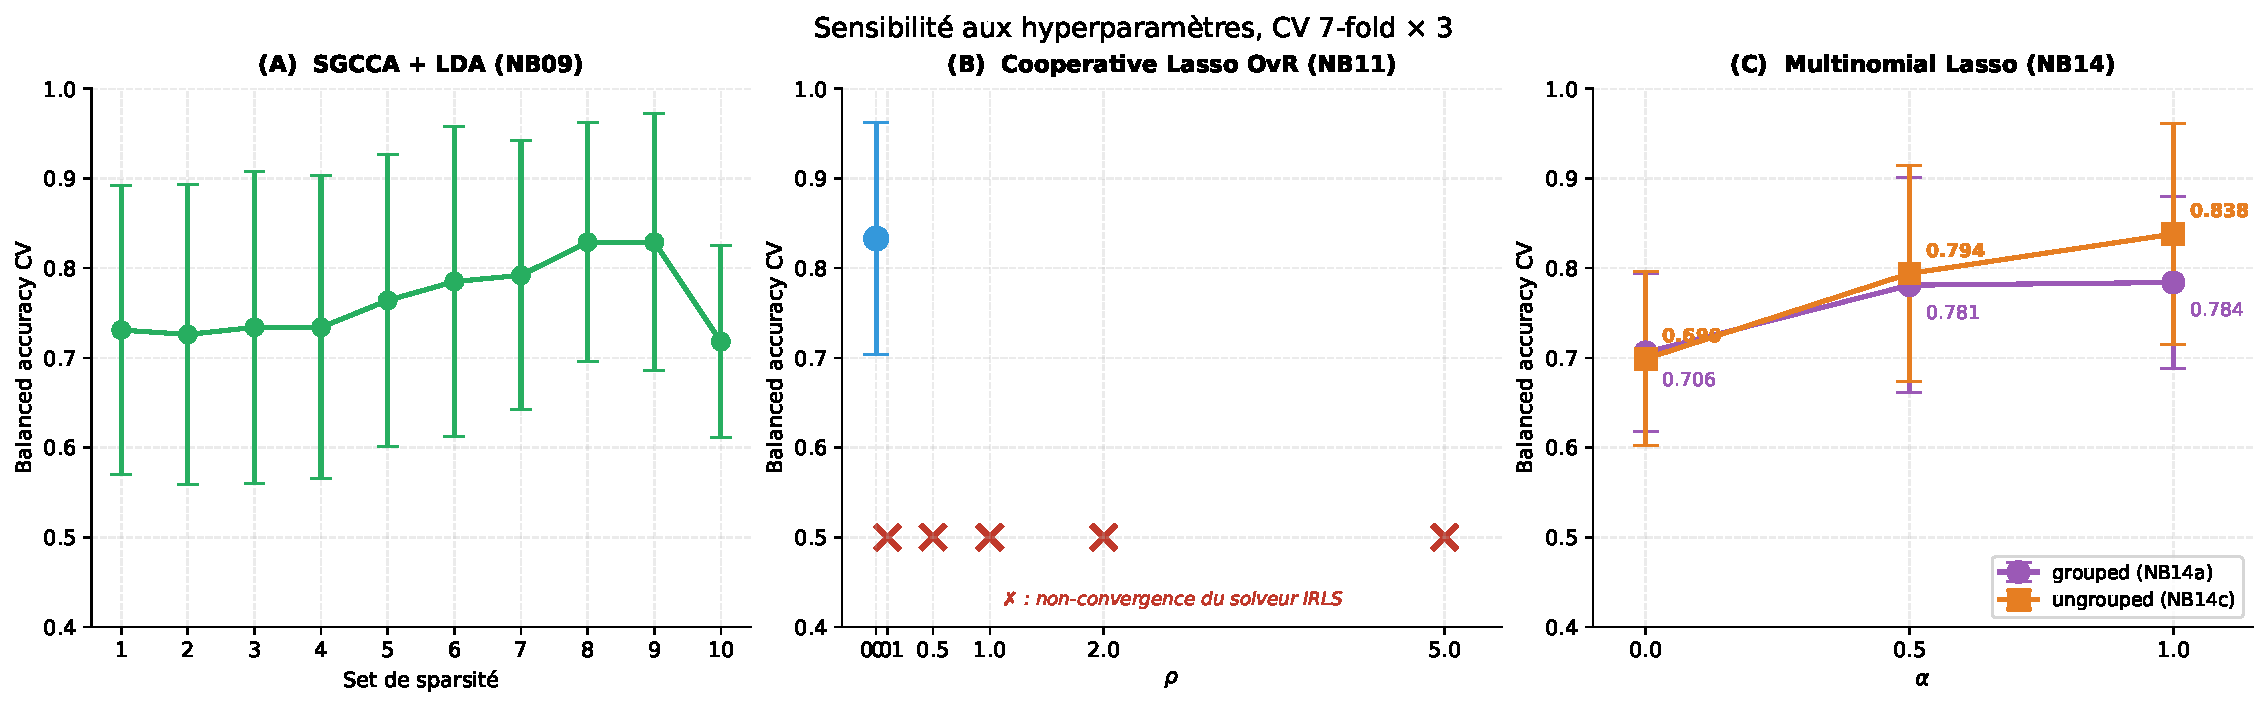
\includegraphics[width=\linewidth]{fig2_hp_sensitivity.pdf}
    \caption{Hyperparameter sensitivity analysis.
        \textbf{(A)} SGCCA + LDA: Sparsity sweep across candidate grid configurations evaluated by \texttt{rgcca\_cv}, showing optimal validation performance at Sets 8 and 9.
        \textbf{(B)} Cooperative Lasso OvR: Agreement penalty sweep ($\rho$); red crosses indicate configurations where the \texttt{multiview} solver failed to converge, leaving only $\rho = 0$ functional.
        \textbf{(C)} Multinomial Lasso: Elastic-Net mixing sweep ($\alpha$) comparing \texttt{grouped} (purple) vs. \texttt{ungrouped} (orange) penalties; at $\alpha = 1$, ungrouped selection yields a $+0.054$ gain in CV balanced accuracy.}
    \label{fig:hp_sensitivity}
\end{figure}

\begin{figure}[H]
    \centering
    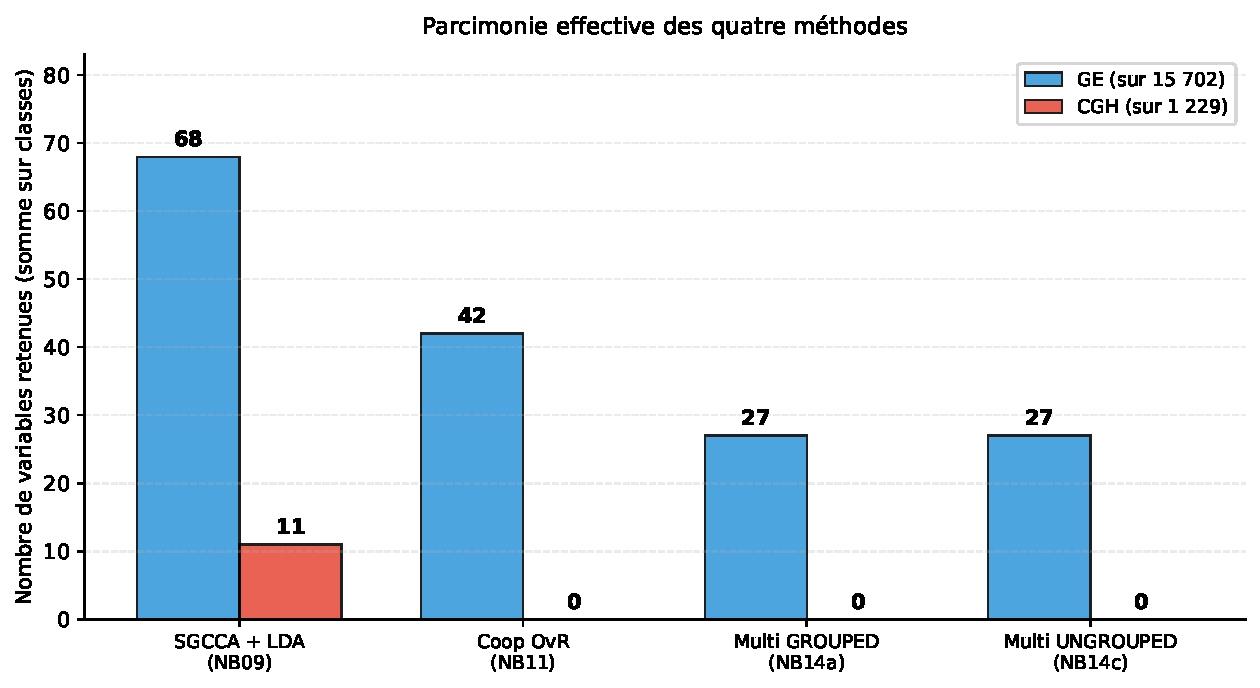
\includegraphics[width=0.9\linewidth]{fig4_sparsity.pdf}
    \caption{Number of retained variables per molecular block across methods.}
    \label{fig:sparsity}
\end{figure}

All data-driven models spontaneously eliminate the entire CGH block; only SGCCA retains $11$ CGH variables because its block-wise constraint $s_{\text{CGH}}$ is structurally enforced.

\begin{figure}[H]
    \centering
    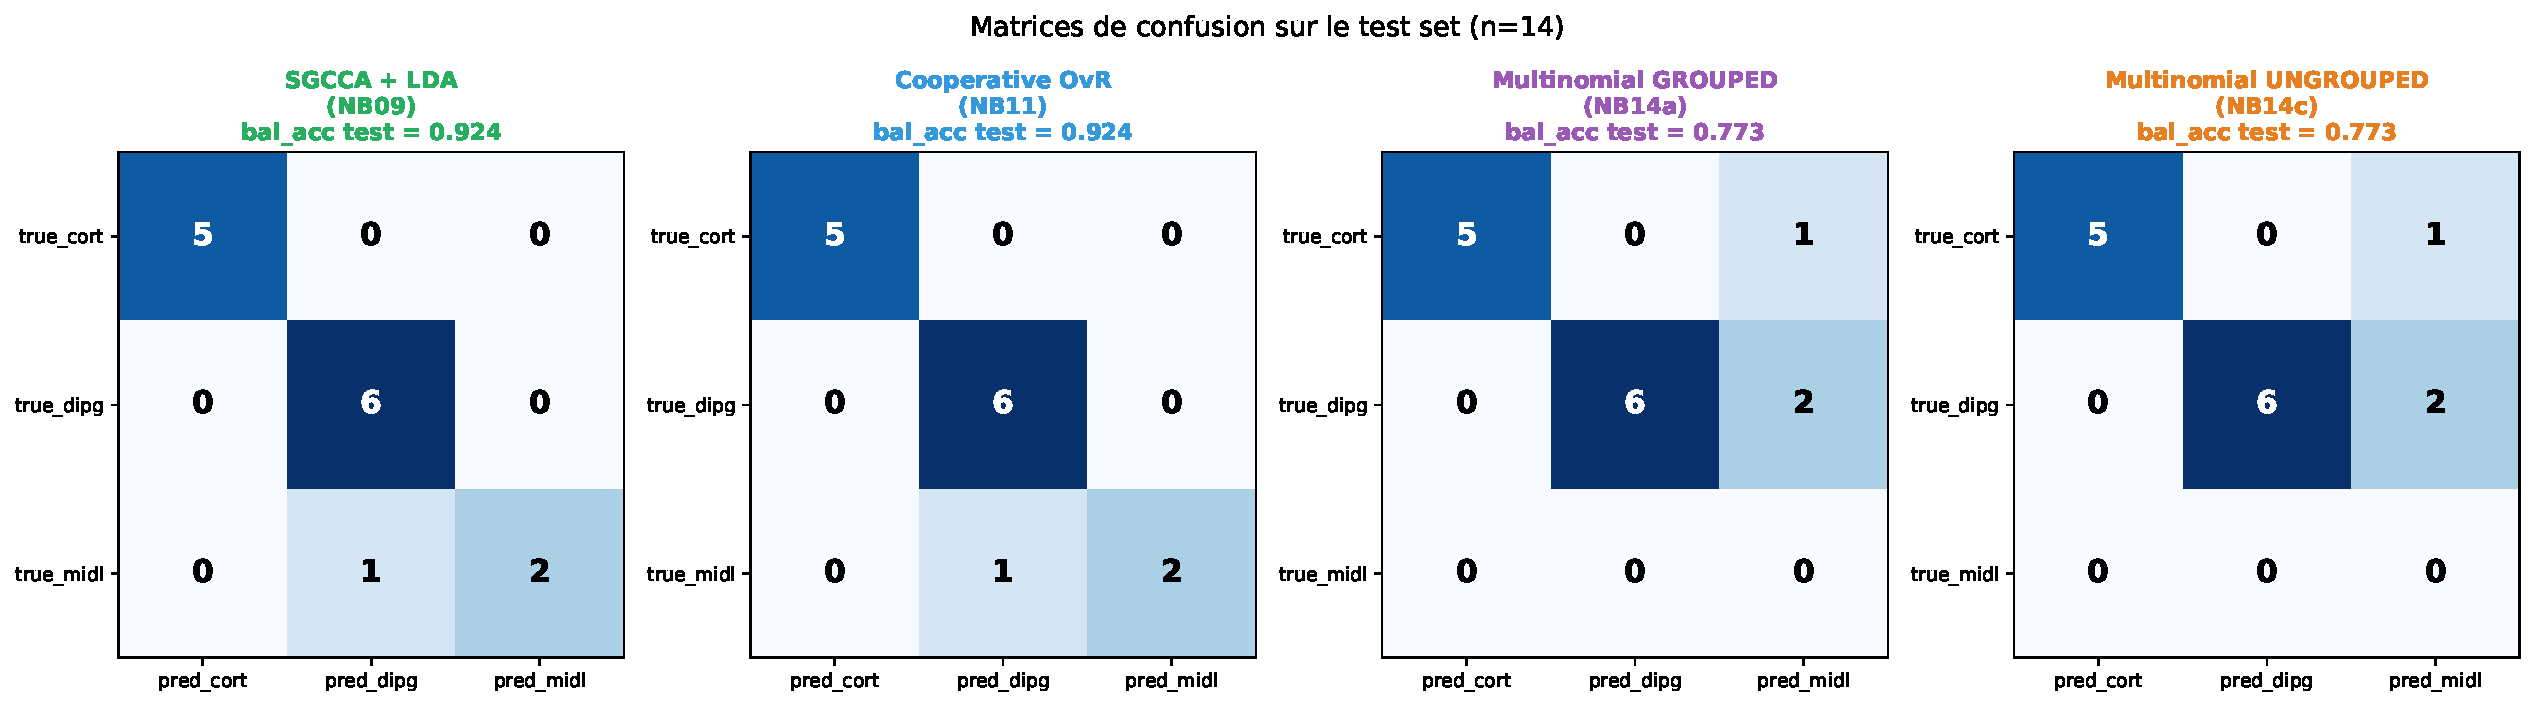
\includegraphics[width=\linewidth]{fig3_confusion.pdf}
    \caption{Test set confusion matrices across evaluated pipelines.}
    \label{fig:confusion}
\end{figure}

All four methods exhibit near-perfect classification on \texttt{cort} and \texttt{dipg}. Discrepancies are driven exclusively by the \texttt{midl} class ($n = 3$ test patients): SGCCA + LDA and Cooperative OvR classify $2/3$ \texttt{midl} tumors correctly, whereas multinomial Lasso variants misclassify all three into \texttt{dipg}.

\begin{figure}[H]
    \centering
    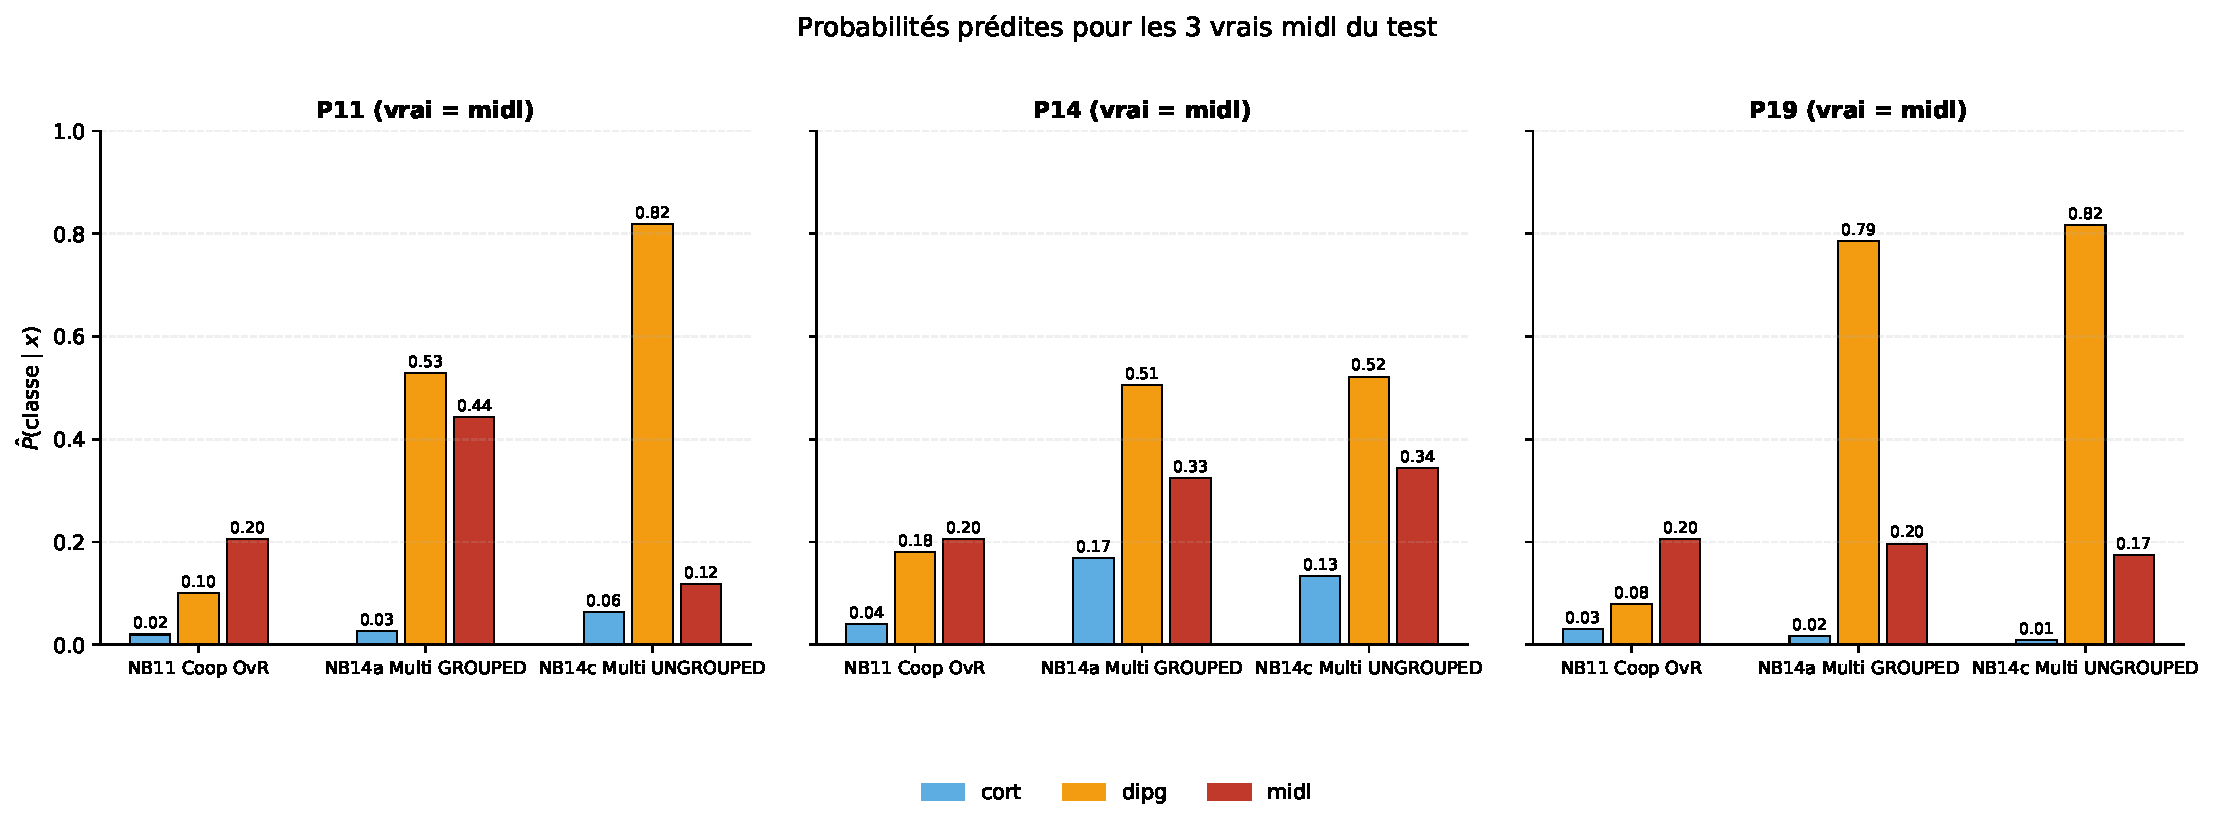
\includegraphics[width=1\linewidth]{fig6_midl_probs.pdf}
    \caption{Predicted class probabilities for test \texttt{midl} patients under One-vs-Rest regression.}
    \label{fig:midl_probs}
\end{figure}

Cooperative OvR predicts a steady baseline probability $\hat P_{\text{midl}} \simeq 0.205$, which dominates by $\arg\max$ for patients P11 and P19 when \texttt{cort} and \texttt{dipg} probabilities are suppressed. Under multinomial models, the sum-to-one constraint forces this probability mass into \texttt{dipg}.

\newpage


\section{Stability and Statistical Validation}
\label{sec:stabilite}

To establish the reliability of our findings, we applied three validation techniques: bootstrap resampling \cite{efron1979bootstrap} and stability selection \cite{meinshausen2010stability} to quantify biomarker reproducibility, and permutation testing \cite{ojala2010permutation} to verify global significance.

\subsection{Feature Selection Stability}

In high dimensions, selected variable sets can be sensitive to sample perturbations. We evaluated selection frequency across $B = 200$ bootstrap resamples (Figure~\ref{fig:stab_bootstrap}). Two patterns emerge:
\begin{itemize}
    \item A core set of GE genes is consistently selected across resamples, forming a stable predictive signature.
    \item The exclusion of the CGH block is stable: no data-driven model selects CGH features across resamples, confirming that its exclusion is genuine rather than an artifact of sample splitting.
\end{itemize}

Applying stability selection with threshold $\pi_{\text{thr}} = 0.6$ controls the expected false discovery rate.

\begin{figure}[H]
    \centering
    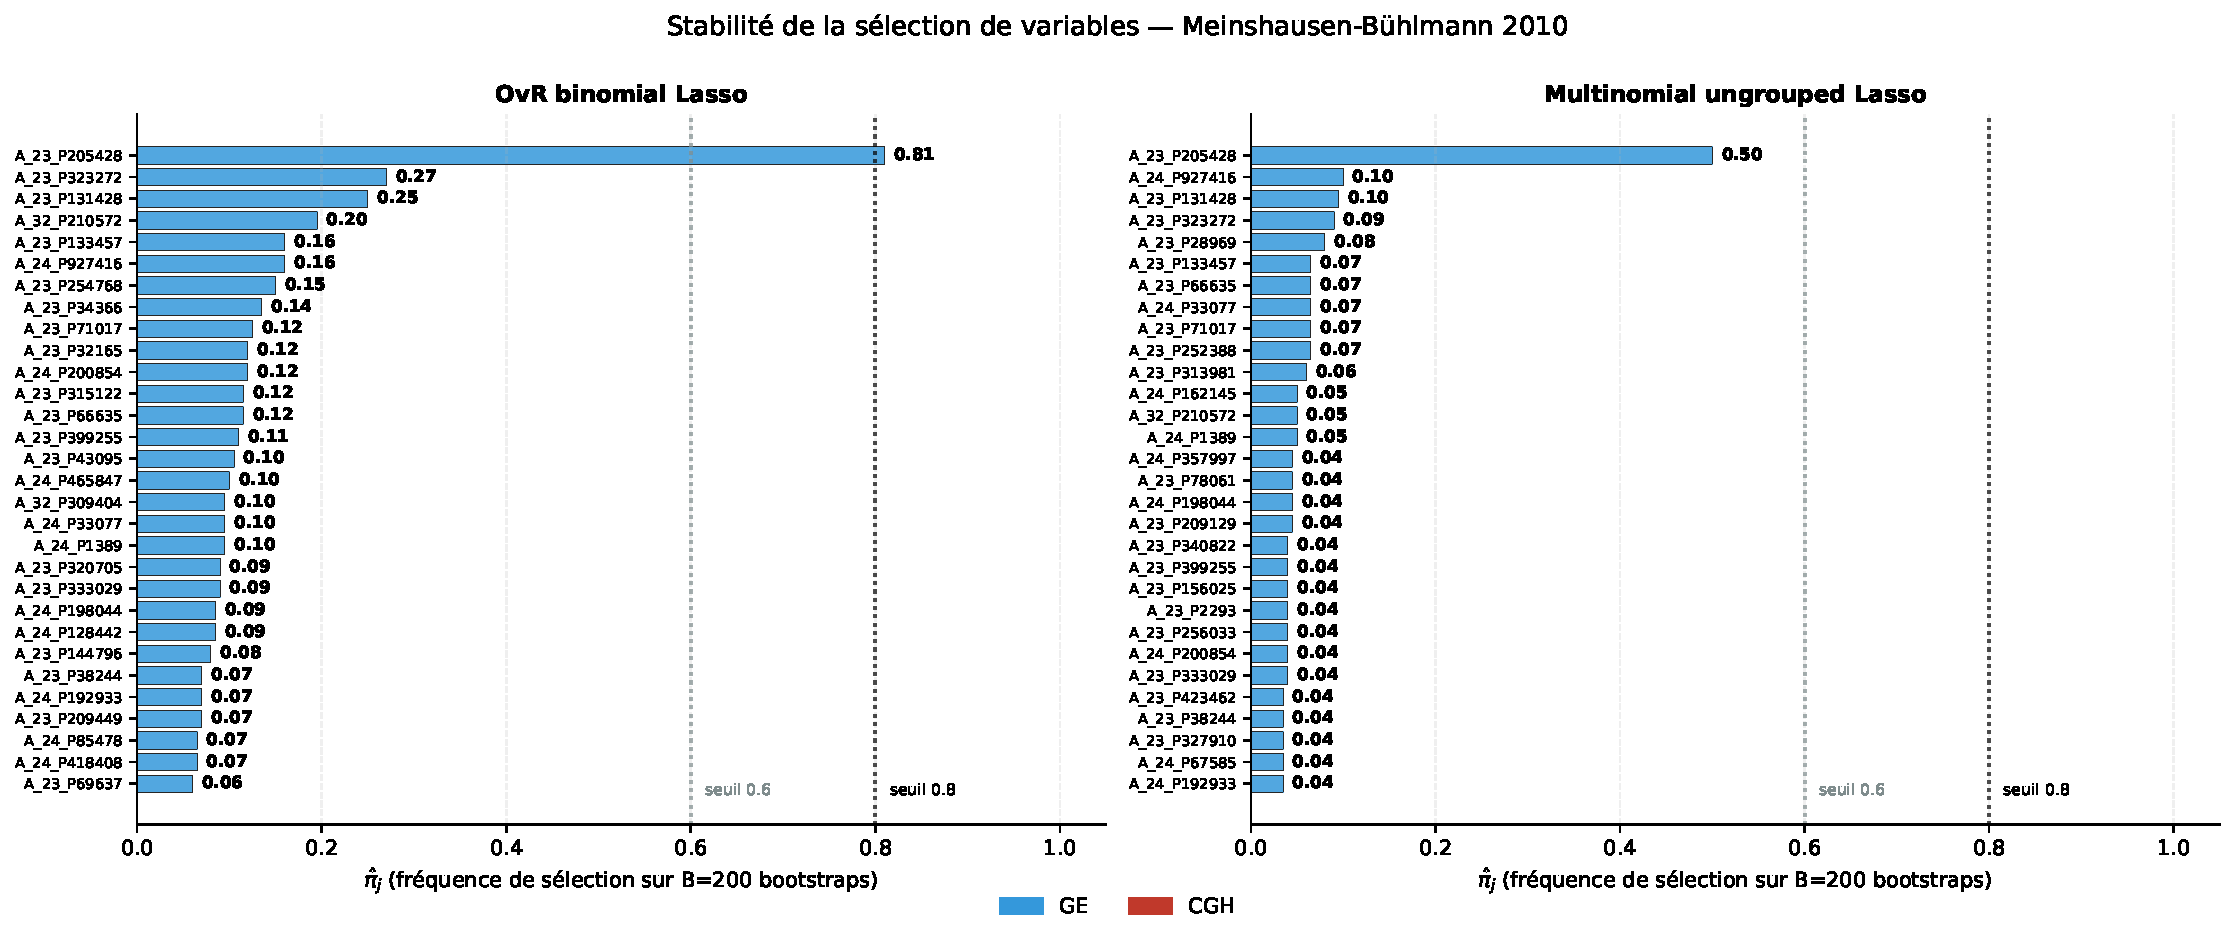
\includegraphics[width=\linewidth]{fig9_stability_bootstrap.pdf}
    \caption{Variable selection frequency across $B = 200$ bootstrap resamples for OvR Lasso. A compact core of GE genes exhibits high selection stability, while most features are selected sporadically.}
    \label{fig:stab_bootstrap}
\end{figure}

\begin{figure}[H]
    \centering
    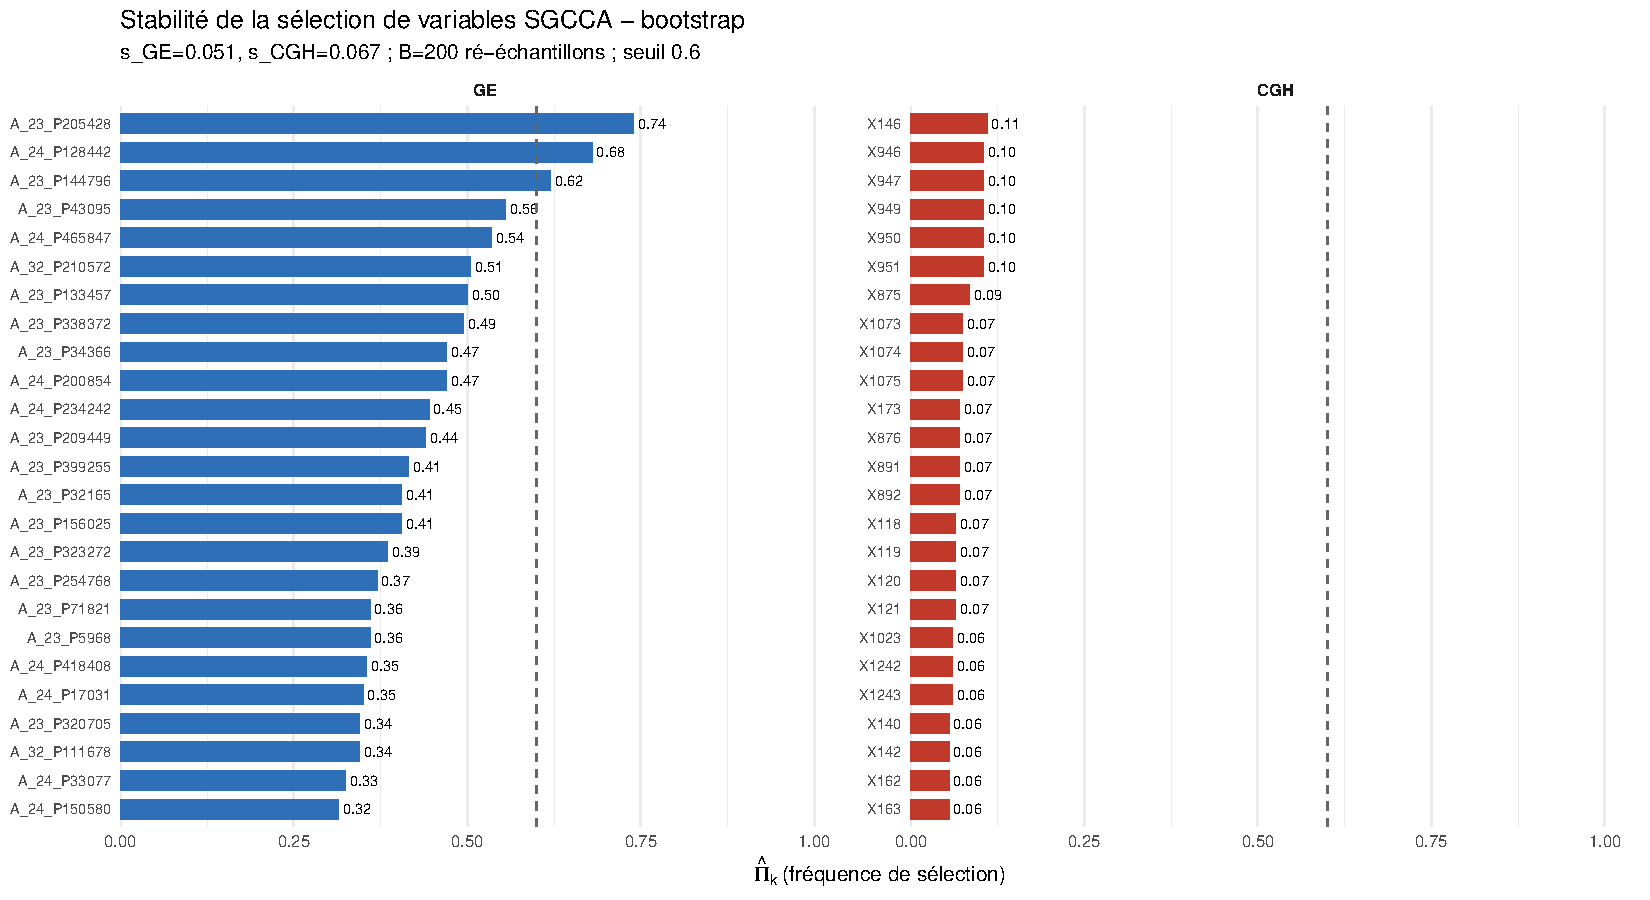
\includegraphics[width=\linewidth]{fig12_sgcca_stability.pdf}
    \caption{Variable selection frequency under SGCCA across $B = 200$ bootstrap resamples ($s_{\text{GE}} = 0.051, s_{\text{CGH}} = 0.067$, threshold $0.6$). Compared to OvR Lasso, selection is more diffuse, with CGH features remaining at low background frequency ($\hat \Pi_k \le 0.11$).}
    \label{fig:sgcca_stab}
\end{figure}

Evaluating SGCCA under bootstrap resampling (Figure~\ref{fig:sgcca_stab}) reveals that whereas OvR Lasso isolates a prominent top marker (\texttt{A\_23\_P205428}, $\hat \Pi_k \approx 0.81$), SGCCA distributes selection weights across a broader spectrum of genes whose frequencies decline gradually from $0.74$ to $0.30$. Only three genes exceed $\pi_{\text{thr}} = 0.6$. The CGH block contributes only diffuse background noise ($\hat \Pi_k \le 0.11$).

\subsection{Statistical Significance via Permutation Testing}

To verify that model accuracy does not reflect overfitting to noise, we executed non-parametric permutation tests \cite{ojala2010permutation}:
\begin{itemize}
    \item \textbf{Null Hypothesis $H_0$}: Class labels are statistically independent of molecular features (expected balanced accuracy $= 1/3$).
    \item \textbf{Alternative Hypothesis $H_1$}: Molecular profiles contain genuine discriminative signal for tumor localization.
\end{itemize}

The test permutes training labels and retrains the entire pipeline from scratch across $B = 500$ iterations. The empirical $p$-value is computed as the proportion of permuted runs achieving a balanced accuracy equal to or greater than that observed on unpermuted data.

All evaluated models achieve an empirical \textbf{$p$-value of $0.002$} (the minimum attainable value for $B = 500$), rejecting $H_0$. The predictive signal is statistically significant.

\subsection{Reproducibility and Synthesis}

All experiments were executed with fixed pseudo-random seeds across cross-validation splits, bootstrap resamples, and solver initializations, guaranteeing exact reproducibility.

In summary, we distinguish between robust findings and fragile aspects:
\begin{itemize}
    \item \textbf{Robust Findings}: The discriminative signal is concentrated entirely within the gene expression (GE) block; the CGH block is uninformative in isolation; \texttt{cort} and \texttt{dipg} tumors are cleanly separable; and global classification accuracy is statistically significant.
    \item \textbf{Fragile Aspects}: The fine-grained ranking between the top two models (SGCCA + LDA vs. OvR Lasso); the exact recall on the rare \texttt{midl} class (which hinges on $1$--$2$ test patients); and the peripheral composition of selected gene lists outside the stable core.
\end{itemize}

\newpage

\nocite{ding2022cooperative,tenenhaus2011rgcca,tenenhaus2014sgcca,meinshausen2010stability,tibshirani1996lasso,zou2005elasticnet,friedman2010glmnet,tibshirani2005fusedlasso,chawla2002smote,efron1979bootstrap,ojala2010permutation}
\section*{References}
\printbibliography[heading=none]
\label{sec:sources}

\end{document}
